\documentclass[10pt,xcolor={usenames},fleqn,mathserif,serif]{beamer}

%%%Usefull link
%tikz-equations:
%http://www.wekaleamstudios.co.uk/posts/creating-a-presentation-with-latex-beamer-equations-and-tikz/

% There are many different themes available for Beamer. A comprehensive
% list with examples is given here:
% http://deic.uab.es/~iblanes/beamer_gallery/index_by_theme.html
% You can uncomment the themes below if you would like to use a different
% one:
%\usetheme{AnnArbor}
%\usetheme{Antibes}
%\usetheme{Bergen}
%\usetheme{Berkeley}
%\usetheme{Berlin}
%\usetheme{Boadilla}
%\usetheme{boxes}
%\usetheme{CambridgeUS}
%\usetheme{Copenhagen}
%\usetheme{Darmstadt}
\usetheme{default}
%\usetheme{Frankfurt}
%\usetheme{Goettingen}
%\usetheme{Hannover}
%\usetheme{Ilmenau}
%\usetheme{JuanLesPins}
%\usetheme{Luebeck}
%\usetheme{Madrid}
%\usetheme{Malmoe}
%\usetheme{Marburg}
%\usetheme{Montpellier}
%\usetheme{PaloAlto}
%\usetheme{Pittsburgh}
%\usetheme{Rochester}
%\usetheme{Singapore}
%\usetheme{Szeged}
%\usetheme{Warsaw}

\hypersetup{pdfpagemode=FullScreen}

\addtobeamertemplate{block begin}{%
  \setlength{\textwidth}{0.95\textwidth}%
  \setlength\abovedisplayskip{0pt}%
}{}


\setbeamertemplate{caption}{\insertcaption}

%% colors
\definecolor{bittersweet}{rgb}{1.0, 0.44, 0.37}
\definecolor{brilliantlavender}{rgb}{0.96, 0.73, 1.0}
\definecolor{antiquefuchsia}{rgb}{0.57, 0.36, 0.51}
\definecolor{violetw}{rgb}{0.93, 0.51, 0.93}
\definecolor{Veronica}{rgb}{0.63, 0.36, 0.94}
\definecolor{atomictangerine}{rgb}{1.0, 0.6, 0.4}
\definecolor{darkgray}{rgb}{0.66, 0.66, 0.66}
\definecolor{brightcerulean}{rgb}{0.11, 0.67, 0.84}
\definecolor{cadmiumorange}{rgb}{0.93, 0.53, 0.18}
\definecolor{ochre}{rgb}{0.8, 0.47, 0.13}
\definecolor{midnightblue}{rgb}{0.1, 0.1, 0.44}
\definecolor{lemon}{rgb}{1.0, 0.97, 0.0}
\definecolor{grey}{rgb}{0.7, 0.75, 0.71}
\definecolor{amber}{rgb}{1.0, 0.75, 0.0}
\definecolor{almond}{rgb}{0.94, 0.87, 0.8}
\definecolor{bf}{RGB}{88, 86, 88}
\definecolor{bb}{RGB}{177, 177, 177}


%%%%%%%%%%%%%%%%%%%%%%%%%%%%%%%%%%% importa pacchetti
\usepackage{usepkg}
%%%%%%%%%%%%%%%%%%%%%%%%%%%%%%%%%%% Funzioni generali
\usepackage{functions}
%http://tex.stackexchange.com/questions/246/when-should-i-use-input-vs-include
\newcommand{\setmuskip}[2]{#1=#2\relax} %%problem usinig mu with calc (req by mathtools) loaded
\usepackage{sources}
%\usepackage{length}
%%%%%%%%%%%%%%%%%%%%%%%%%%%%%%%%%%% Funzioni per questo file main
\usepackage{mathOp}

\def\status{keeptrying}
\def\keeptrying{keeptrying}
\usepackage{LocalF}
%%%%%%%%%%%%%%%%%%%%%%%%%%%%%%%%%


\title{Modi normali di oscillazione del Sole}

% A subtitle is optional and this may be deleted
\subtitle{Struttura interna e modi di oscillazione}

%\author{F.~Author\inst{1} \and S.~Another\inst{2}}
% - Give the names in the same order as the appear in the paper.
% - Use the \inst{?} command only if the authors have different
%   affiliation.

%\institute[Universities of Somewhere and Elsewhere] % (optional, but mostly needed)
%{
% \inst{1}
% Department of Computer Science\\
%  University of Somewhere
%  \and
%  \inst{2}%
%  Department of Theoretical Philosophy\\
%  University of Elsewhere}
% - Use the \inst command only if there are several affiliations.
% - Keep it simple, no one is interested in your street address.

\date{Appello Luglio, \today}
% - Either use conference name or its abbreviation.
% - Not really informative to the audience, more for people (including
%   yourself) who are reading the slides online

\subject{Eliosismologia}
% This is only inserted into the PDF information catalog. Can be left
% out. 

% If you have a file called "university-logo-filename.xxx", where xxx
% is a graphic format that can be processed by latex or pdflatex,
% resp., then you can add a logo as follows:

% \pgfdeclareimage[height=0.5cm]{university-logo}{university-logo-filename}
% \logo{\pgfuseimage{university-logo}}

% Delete this, if you do not want the table of contents to pop up at
% the beginning of each subsection:
%\AtBeginPart[]
%{
%  \begin{frame}<beamer>{Outline}    %\tableofcontents[currentsection]
%  \end{frame}
%}

%\AtBeginDocument{%
%\addtolength\abovedisplayskip{-0.5\baselineskip}%
%\addtolength\belowdisplayskip{-1\baselineskip}%
%\addtolength\abovedisplayshortskip{-0.5\baselineskip}%
%\addtolength\belowdisplayshortskip{-1\baselineskip}%
%}

\makeatletter
\AtBeginPart{%
  \addtocontents{toc}{\protect\beamer@partintoc{\the\c@part}{\beamer@partnameshort}{\the\c@page}}%
}
%% number, shortname, page.
\providecommand\beamer@partintoc[3]{%
  \ifnum\c@tocdepth=-1\relax
    % requesting onlyparts.
    \makebox[6em]{PART #1:} #2
    \par
  \fi
}
\define@key{beamertoc}{onlyparts}[]{%
  \c@tocdepth=-1\relax
}
\makeatother%

\setbeamertemplate{navigation symbols}{}

\makeatletter
\setbeamertemplate{headline}
{
    \leavevmode%
    \hbox{%Refintro
        \begin{beamercolorbox}[wd=.1\paperwidth,ht=2.25ex,dp=1ex,center]{author in head/foot}%
            \hyperlink{intro}{Intro}
        \end{beamercolorbox}%

 \begin{beamercolorbox}[wd=.1\paperwidth,ht=2.25ex,dp=1ex,center]{author in head/foot}%refs Part 1
            \hyperlink{part:MSS}{MSS}
        \end{beamercolorbox}%

 \begin{beamercolorbox}[wd=.2\paperwidth,ht=2.25ex,dp=1ex,center]{author in head/foot}%refs Part 2
            \hyperlink{part:oscillations}{Oscillazioni lineari adiabatiche}
        \end{beamercolorbox}%
        
         \begin{beamercolorbox}[wd=.2\paperwidth,ht=2.25ex,dp=1ex,center]{author in head/foot}%refs Part 3
            \hyperlink{part:inverseproblem}{Problema inverso}
        \end{beamercolorbox}%inverseproblem
        
        \begin{beamercolorbox}[wd=.35\paperwidth,ht=2.25ex,dp=1ex,right]{date in head/foot}%
            %   \usebeamerfont{date in head/foot}\insertshortdate{}\hspace*{2em}
            \insertframenumber{} \hspace*{2ex}  / \hspace*{2ex} \inserttotalframenumber
            \hspace*{2ex} 
        \end{beamercolorbox}}%
        \vskip0pt%
    }
    \makeatother

\AtBeginSection{\frame{\sectionpage}}

% Let's get started
\begin{document}

\addtobeamertemplate{block begin}{\setlength\abovedisplayskip{2pt}\setlength\belowdisplayskip{2pt}\setlength\abovedisplayshortskip{2pt}\setlength\belowdisplayshortskip{2pt}}

\addtobeamertemplate{block begin}{\vspace*{-3pt}}{}
\addtobeamertemplate{block end}{}{\vspace*{-3pt}}

\begin{frame}
  \titlepage
\end{frame}

% Section and subsections will appear in the presentation overview
% and table of contents.
%\frame{\tableofcontents[onlyparts]}

\begin{frame}[label={intro}]{Modi di oscillazione della struttura solare}

Inserire figura sole senza spicchio modi

\end{frame}

\begin{wordonframe}{Intro MSS e i suoi modi}

In questa tesina mi sono occupato dei modi normali gravo-acustici solari cio\'e oscillazioni attorno alla struttura di equilibrio le cui caratteristiche sono determinate dal profilo radiale della densit\'a e velocit\'a del suono. Il gran numero di frequenze osservate impone vincoli stringenti alle caratteristiche del modello solare standard.

Nella prima parte ho considerato analizzato il modello solare standard, nella seconda ho descritto i modi normali adiabatici, in particolare la relazione tra le frequenze dei modi e la struttura solare; infine ho considerato le tecniche che permettono di invertire la dipendenza delle frequenze dalla struttura interna del Sole.

Il modello MSS si basa su leggi di conservazione, valide per qualsiasi stella: le prime 3 equazioni usate per determinare la struttura stellare ... 

\end{wordonframe}



\part{Modello solare e osservabili sismologiche}\label{part:MSS}
\frame{\partpage}

%\begin{frame}{Argomenti}
%  \tableofcontents[part=1,hideallsubsections%,pausesections
%  ]
%  % You might wish to add the option [pausesections]
%\end{frame}


%\section{Equilibrio idrostatico}

\begin{frame}{Leggi di conservazione applicate alla struttura stellare}

%\begin{equation*}
%\tau_{idro}^{\odot}= \sqrt{\frac{R^3}{GM}}\approx\frac{1}{2}(G\overline{\rho})\expy{-\frac{1}{2}}\approx\SI{27}{\minute}
%\end{equation*}

\begin{block}{Simmetria sferica}
Deviazioni da forma sferica trascurabili (campi magnetici, rotazione)
\end{block}

\begin{block}{Conservazione della massa}

\begin{equation*}
%\TDy{t}{\rho}+\nabla\cdot(\rho\vec{v})=0
\TDy{r}{m}=4\pi r^2\rho
\end{equation*}

\end{block}

\begin{block}{Equilibrio idrostatico}

\begin{equation*}
0=-\nabla P(\rho,T)+\rho\vec{g}
%\TDy{r}{P}=-\frac{Gm(r)\rho(r)}{r^2}%\label{eq:fidroequilibrio}
\end{equation*}

\end{block}

\begin{block}{Conservazione energia interna}

\begin{equation*}
\TDy{t}{q}=\epsilon(\rho,T,X_i)-\frac{1}{\rho}\nabla\cdot\vec{F}=\TDy{t}{u}+P\TDof{t}(\frac{1}{\rho})%\label{eq:heatgl}
%&\TDy{r}{L}=4\pi r^2[\rho\epsilon-\rho\TDof{t}u+\frac{P}{\rho}\TDy{t}{\rho}]%\label{eq:fenergyconservation}
\end{equation*}

\end{block}

\begin{block}{Gradiente termico}
\begin{equation*}
\TDy{r}{T}=\nabla\frac{T}{p}\TDy{r}{p}
\end{equation*}
\end{block}

\end{frame}

\begin{wordonframe}{Simmetria sferica, conservazione massa, equilibrio idrostatico, conservazione energia interna (PRIMA LEGGE)}

Le equazioni che descrivono la struttura di una stella ... sono un caso particolare della conservazione della massa, dell'impulso, dell'energia interna.

Considero le deviazioni dalla simmetria sferica (rotazione campo magnetico) come perturbazioni, quindi le trascuro nella descrizione della struttura di equilibrio. 

L'evoluzione di una stella in sequenza principale come il Sole attuale avviene su tempi nucleari quindi assumo equilibrio idrostatico.

Quant'\'e il calore aggiunto per unit\'a di massa?? $\approx\midfrac{E_i}{\tau M}$ In sequenza principale il calore aggiunto per unit\'a di massa \'e trascurabile in qunato i tempi evolutivi sono molto maggiori dei tempi di rilassamento radiativi (tipicamente viene indicato il tempo impiegato ad irradiare l'energia interna).

Per determinare il gradiente termico considero il flusso di energia dalle regioni pi\'u calde alla superficie: oltre al trasporto radiativo devo considerare la convezione presente nella regione esterna per stelle con $M<1.1\msun{}$.

\end{wordonframe}


%\section{Meccanismi di trasporto dell'energia}

\begin{frame}{Trasporto radiativo}

\begin{columns}

\begin{column}{0.5\textwidth}

\begin{block}{Equazione del Trasporto radiativo}
\begin{align*}
%P_{rad}=\int\,d\nu\frac{4\pi}{3c}B_{\nu}=\frac{1}{3}aT^4\\
%\vec{F}=-\frac{4\pi}{3\kappa\rho}\nabla B=-\frac{4\pi}{3\kappa\rho}\nabla B=-\frac{c}{\kappa\rho}\nabla P_{rad}\\
\frac{dI_{\nu}}{\rho\,ds}=j_{\nu}-\kappa_{\nu}I_{\nu}\\
\end{align*}
\end{block}

\end{column}

\begin{column}{0.5\textwidth}

\begin{block}{Equilibrio termodinamico locale}

\begin{align*}
&4\pi j_{\nu}=\kappa_{\nu a}cu(\nu)\\
&B(\nu,T)=\frac{2h\nu^3}{c^2}\frac{1}{\exp{\midfrac{h\nu}{KT}}-1}
\end{align*}

\end{block}

\end{column}

\end{columns}

\begin{equation*}
I_{\nu}=\int_0^{\infty}B_{\nu}(-\tau_{\nu})\exp{-\tau_{\nu}}\,d\tau_{\nu}\approx B(\nu,T)-\frac{1}{\kappa_{\nu}\rho}\nabla_s B(\nu,T)
\end{equation*}

\begin{block}{Relazione tra flusso radiativo e gradiente termico negli interni stellari}

%Il flusso di energia verso la superficie \'e generato da una piccola anisotropia nell'intensit\'a descritta al prim'ordine tramite:
\begin{align*}
%&I_{\nu}=B(\nu,T)-\frac{1}{\kappa_{\nu}'\rho}\nabla_s B(\nu,T)\\
%P_{rad}=\int\,d\nu\frac{4\pi}{3c}B_{\nu}=\frac{1}{3}aT^4\\
%\vec{F}=-\frac{4\pi}{3\kappa\rho}\nabla B=-\frac{4\pi}{3\kappa\rho}\nabla B=-\frac{c}{\kappa\rho}\nabla P_{rad}\\
%&\frac{dI_{\nu}}{\rho\,ds}=\kappa_{a\nu}B_{\nu}(T)-\kappa_{\nu}I_{\nu}\\
%\frac{1}{\kappa}=(\frac{acT^3}{\pi})\expy{-1}\intzi{}\,d\nu\frac{1}{\kappa_{\nu}}\PDy{T}{B(\nu,T)}\label{eq:rosselandopacity}
&\vec{F}=-[\frac{4\pi}{3\rho}\intzi{}\frac{1}{\kappa_{\nu}}\PDy{T}{B(\nu,T)}\,d\nu]\nabla T%=-\frac{c}{\kappa\rho}\nabla P_{rad}
\end{align*}

\end{block}

\begin{block}{Gradiente radiativo}

\begin{equation*}
\nrad{}=\Dcvar{\PDly{P}{T}}{rad}=\frac{3}{16\pi acG}\frac{\kappa l(r)P}{m(r)T^4}%\label{eq:radiativegradient}
\end{equation*}

\end{block}

\end{frame}

\begin{wordonframe}{Relation between energy density u, energy flus in polar direction F and radiation pressure $P_r$ are related to 3 moments of radiation field $I(\theta)$}

\begin{align*}
&I(\theta)=I_0+I_1\cos{\theta}+\ldots\\
&u=\frac{1}{c}\int I(\theta)\,d\Omega=\frac{2\pi}{c}\int_0^{\pi} I(\theta)\sin{\theta}\,d\theta=\frac{4\pi}{c}I_0\\
&F=\int I(\theta)\cos{\theta}\,d\Omega=2\pi\int_0^{\pi} I(\theta)\cos{\theta}\sin{\theta}\,d\theta=\frac{4\pi}{3}I_1\\
&P_r=\frac{1}{c}\int I(\theta)\cos{\theta}^2\,d\Omega=\frac{2\pi}{c}\int_0^{\pi} I(\theta)\cos{\theta}^2\sin{\theta}\,d\theta=\frac{4\pi}{3c}I_0
\end{align*}

\end{wordonframe}

\begin{wordonframe}{Densit\'a di energia fotoni per unit\'a di volume e equilibrio termodinamico radiazione-materia}

Per determinare il gradiente termico considero il flusso di energia dalle regioni pi\'u calde alla superficie: oltre al trasporto radiativo devo considerare la convezione presente nella regione esterna per stelle con $M<1.1\msun{}$.

Il cammino libero medio nell'interno solare \'e molto breve quindi considero la radiazione in equilibro con la materia. La densit\'a di energia dei fotoni per unit\'a di frequenza \'e
\begin{align*}
&u(\nu)=\frac{8\pi h\nu^3}{c^3}\frac{1}{\exp{\midfrac{h\nu}{KT}}-1}\\
&u=aT^4\\
&I(\nu)=\frac{u(\nu)c}{4\pi}
\end{align*}

Equilibrio termodinamico locale (Emissione=assorbimento): opacit\'a dovuta a processi di assorbimento.
\begin{align*}
&4\pi j_{\nu}=\kappa_{\nu a}cu(\nu)\\
&B(\nu,T)=\frac{2h\nu^3}{c^2}\frac{1}{\exp{\midfrac{h\nu}{KT}}-1}
\end{align*}

\end{wordonframe}

\begin{wordonframe}{Emissione spontanea/Indotta}

In realt\'a devo tener conto del\[\frac{\text{Spontaneous emission}}{\text{Total emission}}=1-\exp{-\midfrac{h\nu}{KT}}\]

\[j_{\nu}(\theta)=\kappa_{a,\nu}(1-\exp{-\midfrac{h\nu}{KT}})B_{\nu}(T)+\exp{-\midfrac{h\nu}{KT}})I_{\nu}(T)\]

In LTE si riduce alla legge di Kirkoff.

\end{wordonframe}

\begin{wordonframe}{Trasporto radiativo negli interni stellari: equilibrio termodinamico locale ed espansione $B_{\nu}(-\tau_{\nu})$ al prim'ordine in $\tau_{\nu}$.}

{\small

Infine determino la relazione tra flusso verso la superficie e gradiente termico: oltre al trasporto radiativo devo considerare la convezione presente nella regione esterna per stelle con $M<1.1\msun{}$...

Negli interni stellari il cammino libero medio di un fotone $\invers{(\kappa_{\nu}\rho)}$ \'e molto breve quindi considero localmente equilibrio radiazione-materia.

L'intensit\'a di radiazione attraverso il punto $\vec{P}$ nella direzione $\hat{s}$ \'e determinata dalla somma dei contributi degli strati precedenti 


%Per quanto rigurda il trasporto radiativo la soluzione per l'intensit\'a al raggio r in direzione $\hat{s}$ in condizioni di equilibrio termodinamico locale pu\'o essere approssimata come somma (integrale) dei contributi all'intensit\'a  degli strati sottostanti diminuiti a causa dell'opacit\'a con il termine $\exp{\tau_{\nu}}$.

%Poich\'e negli interni stellari il cammino libero medio di un fotone \'e piccolo (per condizioni solari $\invers{(\kappa\rho)}$) considero l'espansione di $B_{\nu}(-\tau_{\nu})$ al prim'ordine

%(emissivit\'a per unit\'a di frequenza:$B(T)=\frac{ac}{4\pi}T^4$). La soluzione dell'equazione del trasporto radiativo \'e la somma di tutti i contributi $B_{\nu}(-\tau_{\nu})$ pesati dall'esponenziale che descrive l'assorbimento del plasma solare.
%In condizioni tipiche degli interni stellari si pu\'o esprimere l'intensit\'a specifica di radiazione nella direzione $\hat{s}$ come somma del termine isotropo $B_{\nu}(T)$ e del termine lineare nel cammino libero medio del fotone di frequenza $\nu$ che tiene conto della piccola anisotropia nell'intensit\'a specifica tramite $\nabla B_{\nu}(T)$.

%Integrando sulle direzioni uscenti e su tutte le frequenze si ottiene la relazione tra flusso radiativo e gradiente termico.

Integrando su tutte le direzioni e su tutte le frequenze si ottiene la relazione tra flusso e gradiente terico cercata.

La quantit\'a $\frac{1}{\kappa_{\nu}}\PDy{T}{B_{\nu}(T)}$ \'e l'opacit\'a media di Rosseland. Nel calcolo della struttura stellare si usa il gradiente termico espresso in termini della derivata logaritmica della pressione: ho usato la definizione di luminosit\'a e la condizione di equilibrio idrostatico.

}

\end{wordonframe}


\begin{frame}{Instabilit\'a convettiva - Gradiente termico nelle regioni convettive}

\begin{align*}
&\rho\PtwoDy{t}{(\Delta r)}=-g\Delta\rho=-g[\Dcvar{\TDy{r}{\rho}}{e}-\Dcvar{\TDy{r}{\rho}}{amb}]\Delta r=-N^2\Delta r\\
&N^2=g(\frac{1}{\Gamma_1P}\TDy{r}{P}-\frac{1}{\rho}\TDy{r}{\rho})=g(\frac{1}{\densityscale{}}-\frac{g}{c_s^2})%\label{eq:bvfs}
\end{align*}

\begin{columns}

\begin{column}{0.45\textwidth}

\begin{block}{Instabilit\'a convettiva}

\begin{align*}
&N^2<0\\
&\nrad{}>\nad{}
\end{align*}

\end{block}

\begin{block}{Trasporto convettivo}

\begin{align*}
&F=F_c+F_r\\
&F_{con}=\exv{\rho vc_P\Delta T}\\
&l_m=\alpha H_P
\end{align*}

\end{block}

\end{column}

\begin{column}{0.55\textwidth}

\begin{figure}[!h]
    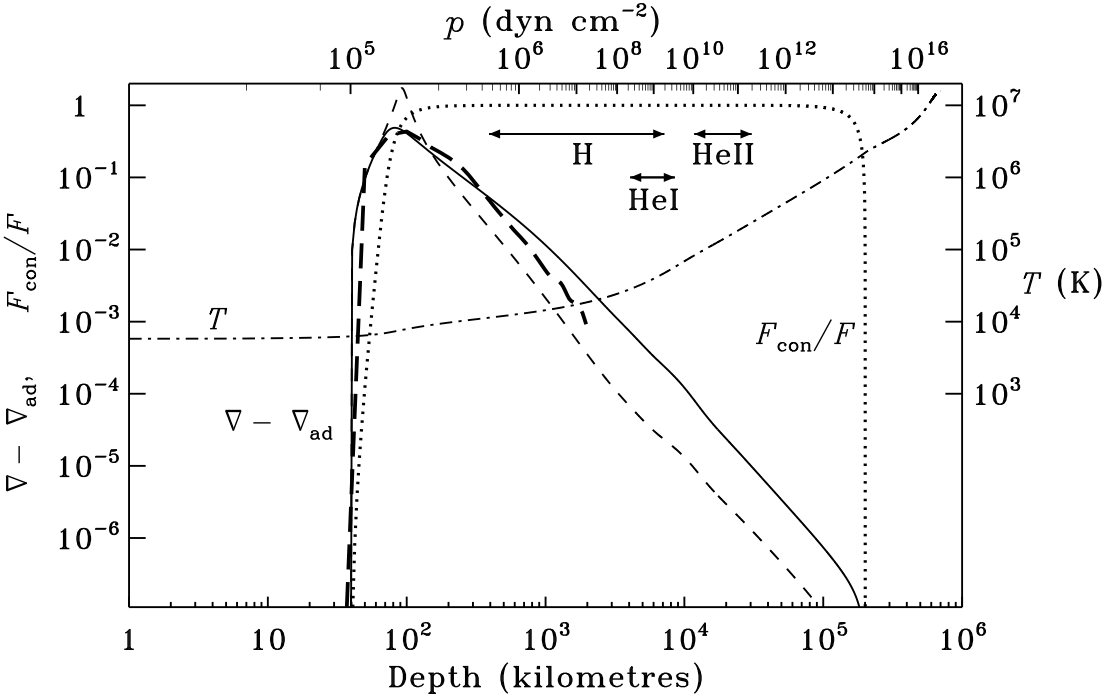
\includegraphics[width=0.99\textwidth,keepaspectratio]{proportionflux}
    \caption{Da \cite{christensen1997effects}.}
\end{figure}


\end{column}

\end{columns}

\end{frame}

\begin{wordonframe}{Instabilit\'a convettiva - Gradiente termico nelle regioni convettive}

La convezione caratterizza le regioni in cui uno spostamento infinitesimo di un blob di gas cresce esponenzialmente a causa della forza di Archimede.

{\small Considero il moto del blob in equilibrio di pressione con l'ambiente: esprimo l'equazione del moto dell'elemento in funzione della frequenza di \bv{} $N^2$. Le regioni stabili, in cui l'equazione del moto descrive un comportamento oscillatorio, sono per $N^2>0$  oppure usando l'equazione di stato per esprimere i gradienti di densit\'a in funzione dei gradienti di temperatura $\nrad{}<\nad{}$.)
}

% e uso l'equazione di stato per esprimere la differenza di densit\'a tra blob e ambiente. Considero in prima approssimazione il moto del blob adiabatico ($dq=c_P\,dT-\frac{\delta}{\rho}\,dP$) (e $\nmu{}\approx0$).

Per determinare il gradiente ambientale nelle regioni convettive esterne, che caratterizzano stelle $M\leq1.1\msun{}$ si usa la teoria della ML. Questa considera l'eccesso di calore trasportato dal moto dell'elemento di gas in equilibrio di pressione con l'ambiente che rilasci il calore dopo aver percorso una lunghezza caratteristica $l_m=\alpha H_P$.

L'efficienza delle regioni convettive esterne \'e quindi un parametro libero determinato tramite calibrazione del modello solare per riprodurre $T_e$.

\end{wordonframe}


%\section{Costruzione modello solare}

\begin{frame}{Modello plasma solare}

\begin{block}{EOS e grandezze termodinamiche. Popolazione di stati atomici.}

\begin{columns}

\begin{column}{0.5\textwidth}

\begin{figure}[!ht]
        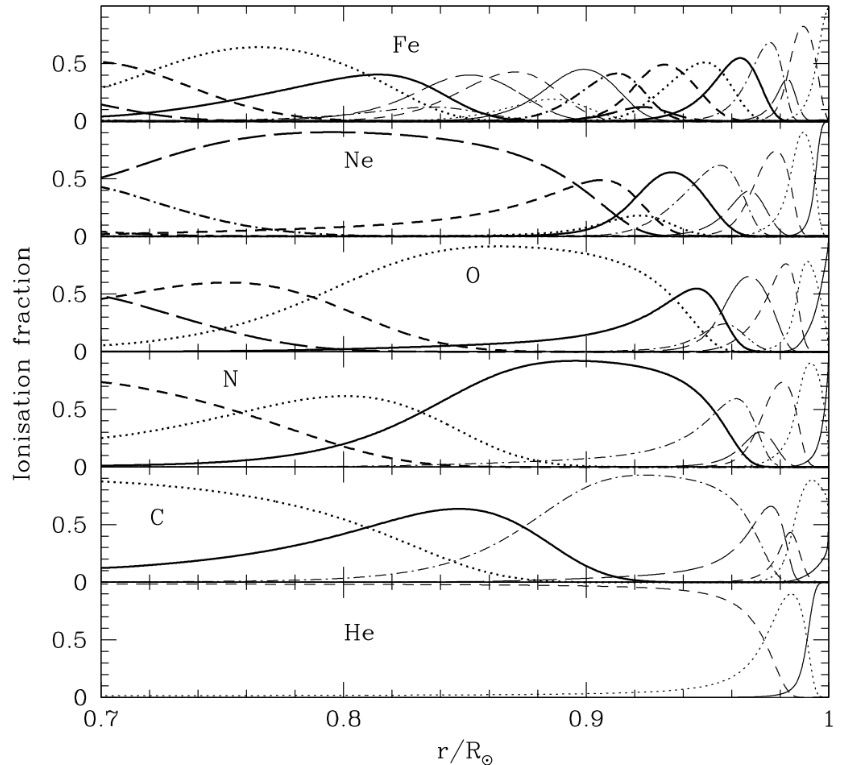
\includegraphics[width=0.9\textwidth,keepaspectratio]{ionfraction}
        \caption{Da \cite{basu2008helioseismology}.}
\end{figure}%


\end{column}

\begin{column}{0.5\textwidth}

%Interazioni coulombiane:
%\begin{equation*}
%\frac{1}{r_D^2}=\frac{4\pi e^2}{kT}\sum_Z Z^2\overline{n}_Z=\frac{4\pi e^2}{kT}N_A\sum_{i}(Z_i^2+Z_i)\frac{\rho X_i}{A_i}
%\end{equation*}
\[\Gamma_1=\left(\PDly{\rho}{P}\right)_s\]

\begin{figure}[!ht]
        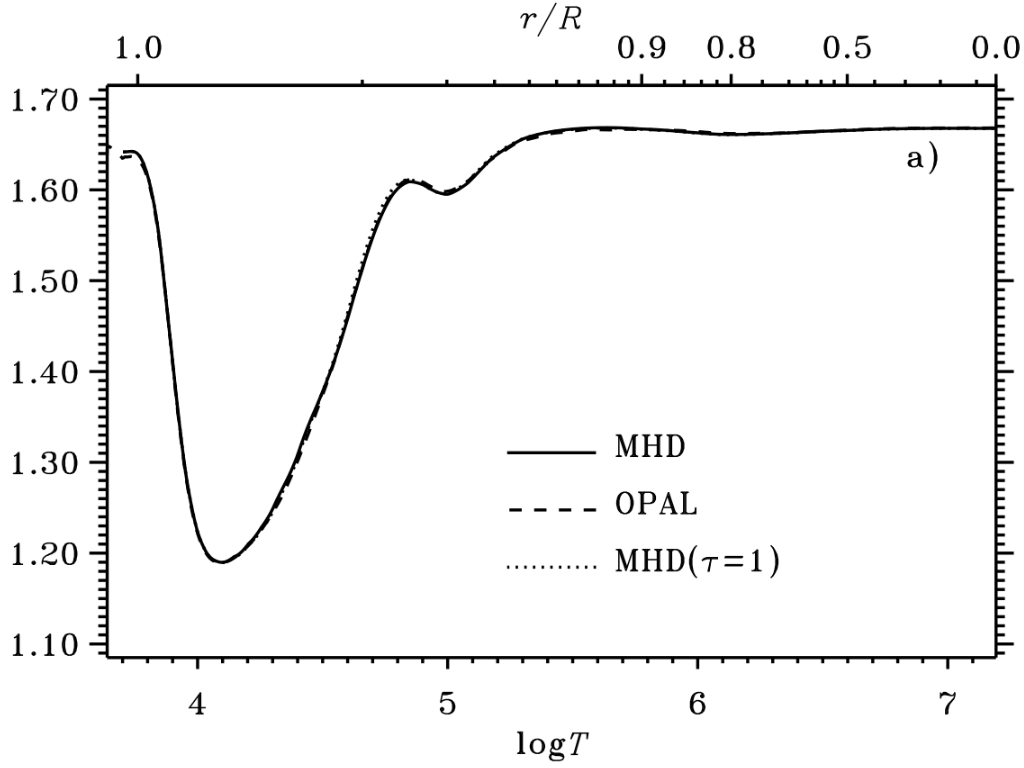
\includegraphics[width=0.9\textwidth,keepaspectratio]{gamma1eos}
        \caption{Da \cite{trampedach2006synoptic}.}
\end{figure}

\end{column}

\end{columns}

\end{block}

\end{frame}

\begin{wordonframe}{Modellizzazione plasma solare}

{\small Per risolvere le equazioni della struttra stellare \'e necessario conoscere le propriet\'a termodinamiche del gas, in particolare l'equazione di stato $P(\rho,T)$.

{\small Nel caso solare l'equazione dei gas perfetti \'e una prima approssimazione poich\'e gli effetti della degenerazione elettronica e delle interazioni coulombiane sono piccoli.}

%Gli approcci pi\'u usati per ricavare un'equazione di stato accurata per il plasma stellare considerano le propriet\'a statistiche di un gas di nuclei ed elettroni oppure di un gas di atomi: nel secondo caso sono necessarie ipotesi ad hoc per tener conto delle perturbazioni ai livelli atomici causati dalle particelle vicine.
\begin{align*}
&P=P_r+P_G=\frac{1}{3}aT^4+\frac{\rho}{\mu}\gasconstant{}T\\
&u=\frac{1}{\rho}\sum_i\int f^{(0)}(\vec{p}_i)\frac{p^2_i}{2m_i}\,d^3p_i=\frac{3}{2}\frac{P}{\rho}%=\frac{3}{2}\frac{\gasconstant{}T}{\mu}
\end{align*}

{\small La principale correzione che tiene conto della natura non puntiforme delle interazioni \'e la correzione coulombiana: le interazioni elettriche modificano la distribuzione delle cariche nel plasma neutro su distanze maggiori di $R_D$ (???cariche su sfera di raggio $R_D$ attorno a ione hanno energia coulombiana e termica paragonabili????).}

Una determinazione accurata delle caratteristiche del plasma solare, in particolare dell'esponente adiabatico $\Gamma_1$, permette di investigare la composizione solare poich\'e nelle regioni di ionizzazione degli elementi pi\'u abbondanti si hanno variazioni dal valore $\Gamma_1=\frac{5}{3}$.

A destra \'e mostrato l'andamento dell'esponente adiabatico calcolato tramite due EOS 

}

\end{wordonframe}


\begin{frame}{Evoluzione chimica: reazioni nucleari e diffusione.}

\begin{block}{Probabilit\'a reazioni di fusione}

\begin{align*}
%&\sigma=\pi\lambdabar^2\Exp{-\dfrac{2\pi Z_1Z_2e^2}{\hbar v}}S(E)\\
%&\exv{\sigma v}=\num{1.3005e-15}[\frac{Z_1Z_2}{AT_6^2}]\expy{\frac{1}{3}}fS_{eff}\exp{-\tau}\si{\cubic\cm\per\second}\\
&\exv{\sigma v}=\num{1.3005e-15}[\frac{Z_1Z_2}{AT_6^2}]\expy{\frac{1}{3}}fS_{eff}\exp{-\num{42.487}(Z_1^2Z_2^2AT_6\expy{-1})\expy{\frac{1}{3}}}\si{\cubic\cm\per\second}\\
%&\tau=\frac{3E_G}{kT}\approx\num{42.487}(Z_1^2Z_2^2AT_6\expy{-1})\expy{\frac{1}{3}}\\
%&E_G=A\expy{\frac{1}{3}}T_7\expy{\frac{2}{3}}\SI{5.665}{\kilo\ev}
\end{align*}

\end{block}

\begin{block}{Sequenza principale}
\[4\cel{H}{1}{}{}\to\cel{He}{4}{}{}+2\APelectron+2\Pnue\]
\[Q_e=\SI{28.6}{\mega\ev}-\exv{\nu}\]
\end{block}


\begin{block}{Diffusione}

\begin{equation*}
\vec{F}_i=-\nabla P_i+n_i(q_i\vec{E}+m_i\vec{g})=\sum_{i\neq j}\int m_{ij}\vec{v}_{ij}C(f_i,f_j)\,d^3v_i (??)%
\end{equation*}

\end{block}

\end{frame}

\begin{comment}
\begin{columns}
\begin{column}{0.5\textwidth}
\end{column}
\begin{column}{0.5\textwidth}
\end{column}
\end{columns}
\end{comment}

\begin{wordonframe}{Evoluzione chimica: reazioni di fusione e diffusione}

Le reazioni nucleari generano la luminosit\'a stellare nella maggior parte della vita di una stella e ne determinano l'evoluzione chimica.

La sezione d'urto di fusione contiene il termine geometrico $\pi\lambdabar^2\propto\frac{1}{E}$ (contributo alla sezione d'urto in onda S: $b=l\lambdabar$),  la probabilit\'a di attraversamento della barriera coulombiana $P_0=\exp{-2\pi\eta}$ e il contributo delle funzoni d'onda nucleari.

Lo schermaggio elettronico aumenta la probabilit\'a di penetrare la barriera coulombiana.

La funzione $\epsilon(T,\rho,X_i)$ descrive la produzione di energia.

La forza per unit\'a di volume agente sulle particelle di specie i (trascurando il gradiente termico) \'e
e in condizioni stazionarie il momento trasferito tramite urti con le altre specie \'e uguale alla forza per unit\'a di volume:

\end{wordonframe}



%\section{Equazioni struttura stellare}

\begin{frame}{Dati osservativi}

\begin{columns}

\begin{column}{0.5\textwidth}

\begin{block}{Et\'a, luminosit\'a, massa, raggio solari}
\begin{tabular}{l|c}
\hline
$\agesun{}$&\SI[separate-uncertainty=true]{4.57\pm0.02e9}{\year}\\
\hline
$\rsun{}$&\SI{695658+-140}{\kilo\meter}\\
\hline
$G\msun$&\num{132712440018+-8}\SI{e9}{\cubic\meter\per\square\second}\\
\hline
$\lsun{}$&\SI{3.8275+-0.0014e33}{\erg\per\second}\\
\hline
\end{tabular}
%\caption[Osservabili solari principali.]{Osservabili solari principali. \cite{haberreiter2008solving}.}
\label{tab:sunO}
\end{block}

\end{column}

\begin{column}{0.5\textwidth}

\begin{block}{Composizione chimica}

%\begin{itemize}[noitemsep,topsep=0pt,parsep=0pt,partopsep=0pt]
Righe di assorbimento della fotosfera.

\begin{table}[]

\pgfplotstabletypeset[
every head row/.style={
before row={\toprule},
after row={\midrule}},
every nth row={2}{before row=\midrule},every last row/.style={after row=\bottomrule},
every first column/.style={column type/.add={|}{}},
every last column/.style={column type/.add={}{|}},
%columns/x/.style = {column type/.add={|}{}},
columns/zx/.style = {column type/.add={|}{}},
display columns/0/.style={column name={}},
%display columns/1/.style={column name={$X$}},
%display columns/2/.style={column name={$Y$}},
%display columns/3/.style={column name={$Z$}},
display columns/1/.style={column name={$\left(\frac{Z}{X}\right)_{ph}$}},
%display columns/5/.style={column name={$X$}},
%display columns/6/.style={column name={$Y$}},
%display columns/7/.style={column name={$Z$}},
%display columns/8/.style={column name={$\frac{Z}{X}$}},
create on use/authors/.style={create col/set list={
%Anders \& Grevesse (1989),Grevesse \& Noels (1993),
Grevesse et al. (1998),Lodders (2003),Asplund et al. (2005),Lodders et al. (2009),\cite{asplund2009chemical},\cite{caffau2011solar}}},
columns/authors/.style={string type},
columns={authors,zx},
/pgf/number format/precision=4
     ]{asplund.txt} %%%
%\captionof{table}{Metallicit\'a attuale determinata da varii autori.}\label{tab:Zhistory}
\end{table}

\end{block}

\end{column}

\end{columns}

\begin{block}{Determinazione dell'efficienza della convezione esterna, dell'abbondanza di elio iniziale e degli altri elementi}

\end{block}

\end{frame}

\begin{wordonframe}{Costruzione del MSS e vincoli}

La costruzione di un modello solare \'e molto meno incerta rispetto a un modello di una stella generica data la mole di informazioni disponibili. Conosciamo con grande accuratezza la distanza tramite lo studio delle orbite dei corpi celesti attorno al Sole, l'et\'a di formazione del sistema solare tramite studio dei meteoriti, la luminosit\'a, e il raggio tramite la misura delle dimensioni apparenti del disco solare.

Inoltre \'e possibile determinare la composizione solare della fotosfera supposta identica a quella della zona convettiva tramite l'analisi delle righe di assorbimento nell'atmosfera.

Le righe di assorbimento dell'elio si formano nelle regioni pi\'u esterne dell'atmosfera dove non \'e ovvia la relazione con la composizione della fotosfera quindi il metodo pi\'u accurato per determinare l'abbondanza di elio \'e tramite calibrazione del modello solare.

L'incertezza sul contenuto di metalli \'e dovuta alle difficolt\'a insite nella descrizione dell'atmosfera: come si vede dalla tabella a destra la disponibilit\'a di modelli pi\'u accurati nelle assunzioni fisiche ha portato a un'abbassamento della metallicit\'a. 

\end{wordonframe}

\begin{frame}{Equazioni della struttura solare}

%Determino la struttura solare integrando numericamente le equazioni fondamentali della struttura stellare
\begin{subequations}%\label{subeqn:stellarstructure}
\begin{align*}
&\TDy{r}{m}=4\pi r^2\rho\\
&\TDy{r}{P}=-\frac{Gm(r)\rho(r)}{r^2}\\
&\TDy{r}{T}=\nabla\frac{T}{p}\TDy{r}{p}\\
&\TDy{r}{L}=4\pi r^2[\rho(\epsilon-\epsilon_{\nu})-\rho\TDof{t}u+\frac{P}{\rho}\TDy{t}{\rho}]
\end{align*}
\end{subequations}
%con $v_i$ velocit\'a di diffusione specie i. Ottengo il profilo radiale delle grandezze $\{P,m,T,L,X_i\}$, note la metallicit\'a iniziale Z, l'equazione di stato $P(\rho,T,X_i)$, l'opacit\'a $\kappa(P,T,X_i)$, il rate di produzione di energia nucleare per grammo $\epsilon(P,T,X_i)$.

\begin{columns}

\begin{column}{0.3\textwidth}
Condizioni al bordo:
\end{column}

\begin{column}{0.5\textwidth}
\begin{itemize}
    \item Superficie: $T_e$, $P_{atm}$
    \item Centro: $l(r=0)$, $m(r=0)$.
\end{itemize}

\end{column}

\end{columns}

\begin{block}{Evoluzione del modello solare}

\begin{equation*}
\PDy{t}{n_i}+\frac{1}{r^2}\PDof{r}(r^2n_iv_i)=\Dcvar{\PDy{t}{n_i}}{Nucl}%\label{eq:difffusionchange}
\end{equation*}

\end{block}

\end{frame}

\begin{frame}{Calibrazione modello solare}

\begin{block}{Abbondanze elio iniziale}
Un maggiore peso molecolare medio comporta un maggiore temperatura nel core di fusione
\end{block}

\begin{block}{efficienza convezione}
Mixing length $l_m=H_p\alpha$
\end{block}

\begin{block}{diffusione}
\[\left(\frac{Z}{X}\right)_{\odot}\]
\end{block}

\end{frame}

\begin{wordonframe}{Soluzione equazioni modello solare}

Integro numericamente per la struttura solare con 2 condizioni in superficie per $T_e$ e $P$ e due condizioni al centro per $l$ e $m$ con metallicit\'a e abbondanza di elio da determinare.

L'evoluzione chimica del core di fusione comporta un aumento di temperatura che avviene su tempi-scala molto maggiori dei tempi caratteristici per trasporto radiativo quindi la struttura del modello solare \'e stazionaria.

La presenza di gradienti di concentrazione, di pressione e termici causano fenomeni di diffusione. La velocit\'a di diffusione \'e determinata supponendo il processo stazionario cio\'e la forza per unit\'a di volume agente sulla specie i \'e bilanciata dal trasperimento di impulso negli urti con le altre specie.

\end{wordonframe}

\begin{wordonframe}{Abbondanza di elio attuale e diffusione - mixing length}

Vario il valore primordiale di Y finoch\'e il modello evoluto all'et\'a attuale riproduce la luminosit\'a osservata. L'abbondanza di elio determinata tramite calibrazione \'e afflitta dalle incertezze su l'efficienza della fusione, l'et\'a del Sole, la luminosit\'a attuale, l'opacit\'a.

La metallicit\'a primordiale \'e determinata dalla metallicit\'a attuale tenendo conto della diffusione.

L'efficienza della convezione determina il gradiente nella regione convettiva esterna per riprodurre $T_e$ attuale.

Determino i due parametri Y e $\alpha$ (efficienza trasporto convettivo) in modo che il modello riproduca a $\agesun{}$ la luminosit\'a attuale e la temperatura efficace attuale.

\begin{block}{Abbondanza iniziale di elio}

Il modello evoluto a $\agesun{}$ riproduce la luminosit\'a attuale $\lsun{}$

\end{block}

\begin{block}{Efficienza convezione}

Mixing length $l_m=H_p\alpha$.

Il modello evoluto a $\agesun{}$ riproduce la temperatura effettiva attuale $T_e$

\end{block}

\begin{block}{Diffusione: matching fra composizione attuale del MSS e composizione fotosferica}

\end{block}

\end{wordonframe}

\begin{frame}{Struttura del MSS}

\begin{figure}[!h]
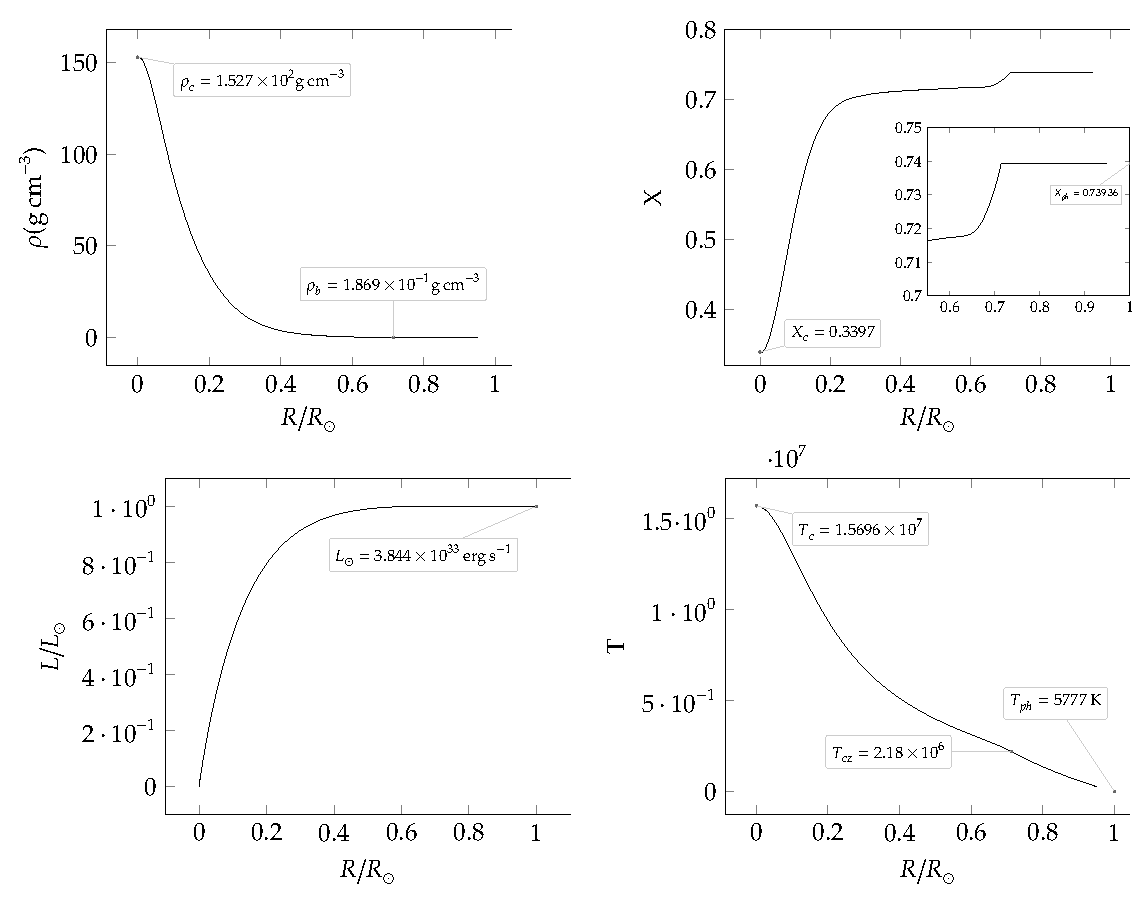
\includegraphics[width=0.75\textwidth,trim=4 4 4 4,clip]{BP00-SSM-R}
\caption{Dati da \cite{BP2000}.}
\end{figure}

\end{frame}

\begin{wordonframe}{Struttura del modello solare - Grandezze sismologiche}

I grafici mostrano il profilo radiale della densit\'a, abbondanza di idrogeno, temperatura e luminosit\'a.

Il profilo dell'abbondanza di idrogeno \'e determinato dalle reazioni di fusione e dalla diffusione, si assume che i moti convettivi rendano la regione convettiva chimicamente omogenea.

La discontinuit\'a nel gradiente termico alla base della zona convettiva \'e evidente nel grafico del profilo termico.

\end{wordonframe}

\begin{frame}{Velocit\'a del suono calcolato tramite MSS}

\begin{figure}[!ht]
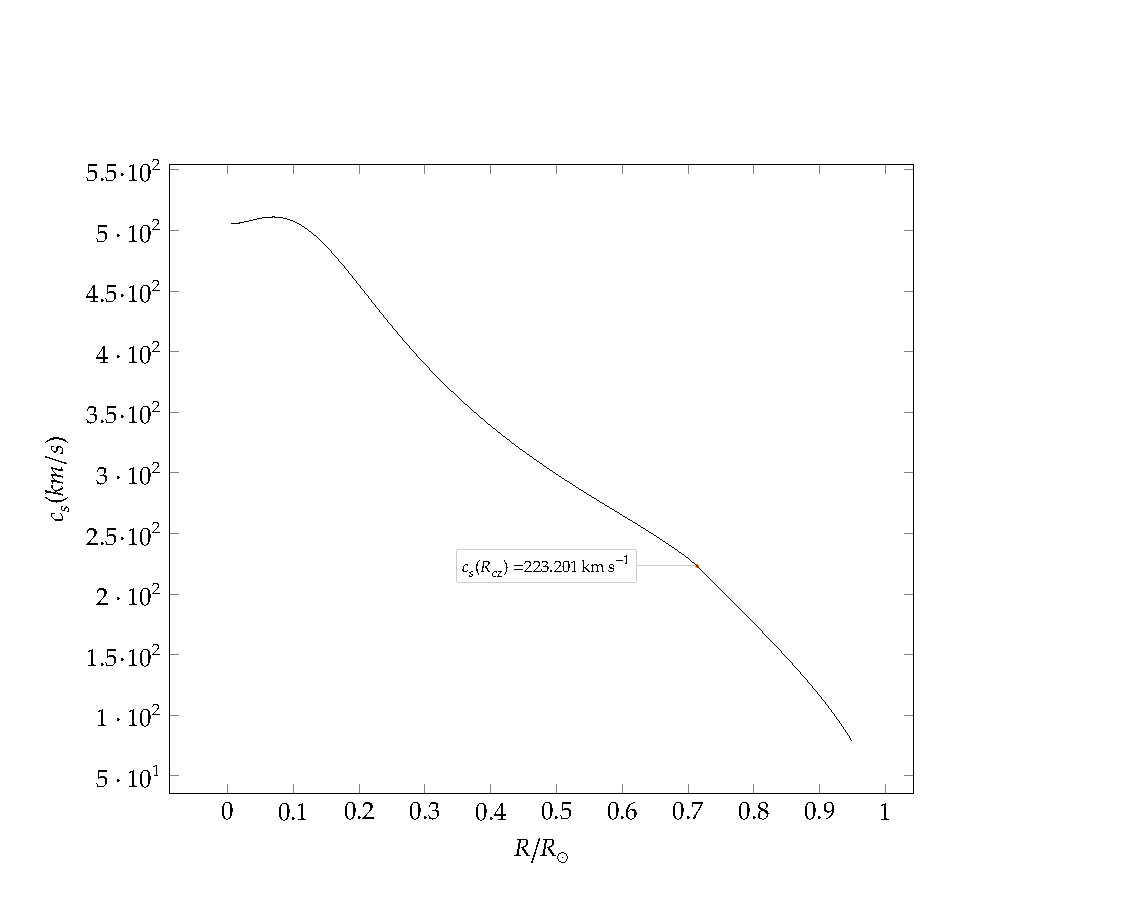
\includegraphics[width=0.9\textwidth]{BP00-cs}
\end{figure}

\end{frame}

\begin{wordonframe}{Profilo radiale della velocit\'a del suono determinato tramite MSS}

In figura abbiamo il profilo della velocit\'a del suono del modello solare precedente.

\end{wordonframe}


\part{Oscillazioni della fotosfera con grande coerenza spaziale e temporale - Modi normali di cavit\'a risonanti dell'interno solare}\label{part:oscillations}

\frame{\partpage}

%\begin{frame}{Argomenti}
%  \tableofcontents[part=2,hideallsubsections%,pausesections
%  ]
  % You might wish to add the option [pausesections]
%\end{frame}

%\section{Modi normali della struttura solare}

\begin{frame}{Modi normali: perturbazioni di una struttura a simmetria sferica}
\begin{block}{Equazione del moto perturbato linearizzata}
\begin{equation*}
\rho_0\TDof{t}\vec{v}=\rho_0\PtwoDy{t}{\vec{\xi}}=-\nabla P'+\rho_0\vec{g}'+\rho'\vec{g}_0%\label{eq:emper}
\end{equation*}
\end{block}
\begin{block}{Equazione di continuit\'a e del moto perturbate}
\begin{equation*}
\rho'+\div{(\rho_0\vec{\xi})}=0%\label{eq:contper}
\end{equation*}
\end{block}
\begin{block}{Condizione di moto adiabatico}
\begin{equation*}
P'+\vec{\xi}\cdot\nabla P_0=\frac{\Gamma_{1,0}P_0}{\rho_0}(\rho'+\vec{\xi}\cdot\nabla\rho_0)%\label{eq:adper}
\end{equation*}
\end{block}
\end{frame}

\begin{wordonframe}{Determinazione del moto perturbato}

L'equazione del moto nel SR solidale con l'elemento di gas linearizzata nella perturbazione insieme alla condizione di adiabaticit\'a del moto e la continuit\'a della massa, sempre al termine lineare nella perturbazione, sono un sistema di 5 equazioni in 5 incognite che con le opportune condizioni al bordo determina i modi di oscillazione adiabatici della struttura solare.
Considero uno spostamento infinitesimo $\vec{\xi}$ dalla posizione di equilibrio di un elemento di gas: la forza agente sull'elemento \'e determinata da pressione densit\'a e accelerazione di gravit\'a a $\vec{r}+\vec{\xi}$. Ottengo l'equazione del moto perturbata al prim'ordine nelle perturbazioni.

Le quantit\'a primate sono perturbazioni euleriane e $\vec{g}'=-\nabla\Phi'$ e $\nabla^2\Phi'=4\pi G\rho'$.

Completo il sistema con l'equazione di continuit\'a e la condizione di moto adiabatico. La condizione di adiabaticit\'a \'e giustificata perch\'e il periodo dei modi \'e molto minore del tempo di rilassamento radiativo e dei tempi scala di generazione di energia.

\end{wordonframe}

\begin{frame}{Modi normali struttura sferica}

\begin{block}{Onde stazionarie}
\begin{align*}
&Y_{lm}(\theta,\phi)=(-)^mc_{lm}P_l^m(\cos{\theta})\exp{im\phi}\\
&(\rho',P',\Phi')=\exp{i\omega t}[\rho'(r),P'(r),\Phi'(r)]Y_l^m
\end{align*}
\end{block}

\begin{block}{Componente tangenziale dello spostamento perturbato}

\begin{align*}
&\vec{\xi}=\exp{i\omega t}(\xi_r(r),\frac{\xi_h(r)}{L}\PDof{\theta},\frac{\xi_h(r)}{L\sin{\theta}}\PDof{\phi})Y_l^m(\theta,\phi)\\
&\xi_h(r)=\frac{L}{r\omega^2}(\frac{P'(r)}{\rho_0}+\Phi'(r))
\end{align*}

\end{block}

\end{frame}

\begin{wordonframe}{Onde stazionarie simmetria sferica}

Cerco soluzioni della forma di onde stazionarie per le perturbazioni scalari e data la simmetria sferica con dipendenza spaziale descritta tramite armoniche sferiche. Utilizzo l'equazione del moto perturbato per mostrare che $\rot{\vec{\xi}}$ non ha componenti radiali: la dipendenza spaziale \'e determinata da un'ampiezza per lo spostamento radiale e un'ampiezza per lo spostamento tangenziale. Applicando la componente tangenziale dell'operatore divergenza all'equazione del moto si trova l'ampiezza tangenziale. 

Questo \'e il sistema che determina i modi normali con le opportune condizioni al bordo: ha soluzioni per $\omega_{nlm}$ discrete.

\end{wordonframe}

\begin{frame}{Modi normali: sistema equazioni fondamentale}

\begin{block}{Modi normali: frequenze discrete dei modi}

\begin{subequations}%\label{eigenomega}
\begin{align*}
&\frac{1}{r^2}\TDof{r}(r^2\xi_r)-\frac{\xi_rg}{c^2}+\frac{1}{\rho_0}(\frac{1}{c^2}-\frac{l(l+1)}{r^2\omega^2})P'-\frac{l(l+1)}{r^2\omega^2}\Phi'=0\\
&\frac{1}{\rho_0}(\TDof{r}+\frac{g}{c^2})P'-(\omega^2-N^2)\xi_r+\TDy{r}{\Phi'}=0\\
&\frac{1}{r^2}\TDof{r}(r^2\TDy{r}{\Phi'})-\frac{l(l+1)}{r^2}\Phi'-\frac{4\pi G\rho_0}{g}N^2\xi_r-\frac{4\pi G}{c^2}P'=0
\end{align*}
\end{subequations}

Condizioni al contorno:

Soluzioni regolari per $r=0$: $P'=0$, $\Phi'=0$.

La condizione di non propagazione oltre la fotosfera: $\Lvar{P}=P'+\xi_r\TDy{r}{P}=0$.

\end{block}

\begin{block}{Approssimazione di Cowling.}
\[\Phi'=0\]
\end{block}

\end{frame}

\begin{wordonframe}{Spettro dei modi: frequenze discrete}

Questo \'e il sistema che determina i modi normali: ha soluzioni per $\omega_{nlm}$ discrete. Le condizioni al bordo richiedono regolarit\'a delle perturbazioni in 0 e riflessione totale delle perturbazioni alla superficie solare. $(l,m)$ caratterizzano la dipendenza angolare dei modi mentre n \'e l'ordine radiale che identifica il numero di zeri radiali del vettore spostamento.

Le frequenze sono $2l+1$ degeneri perch\'e il sistema non dipende da m.

L'approssimazione di Cowling, valida per grandi l o n (uso la soluzione dell'equazione di Poisson per $\Phi'$), consiste nel trascurare la perturbazione al potenziale gravitazionale, restringendosi quindi alle prime 2 equazioni.

\end{wordonframe}

\begin{frame}{Spettro delle oscillazioni adiabatiche}

\begin{columns}

\begin{column}{0.5\textwidth}
\begin{tikzpicture}
\node (inertia) at (0,0) {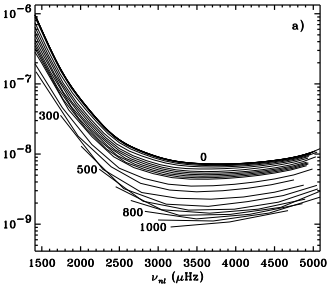
\includegraphics[keepaspectratio,width=0.9\textwidth]{Inertianl}};
\node [below=2mm of inertia.south] {\parbox{0.85\textwidth}{\captionof{figure}{Da \cite{dal03notes}.}}};
\node [left=2mm of inertia.west,rotate=90] {$I_{nl}$};
\end{tikzpicture}
\begin{align*}
%&E_k^{nl}=\frac{1}{2}\int_V|\vec{v}|^2\rho_0\,dV=\frac{\omega_{nl}^2}{2}\int_V|\vec{\xi}_{nl}|^2\rho_0\,dV\\
&\bar{E_k^{nl}}=\frac{1}{\Pi}\int_0^{\Pi}\int\frac{1}{2}\rho_0|\dvec{\xi}_{nl}|^2\,d^3x\,dt=\frac{1}{2}M_{\odot}I_{nl}V_{nl}^2\\
&I_{nl}=\frac{1}{\msun{}A_{nl}^2}\int_V\,d^3x\rho_0\vec{\xi}_{nl}\vec{\xi}_{nl}^*%\label{eq:normalizedinertia}\\
%&\exv{\vec{\xi}(R)\vec{\xi}^*(R)}
%&M_{nl}=I_{nl}\msun{}\intxt{inoltre ho introdotto lo spostamento quadratico medio superficiale}
%&A_{nl}^2=\delta r|_{rms}^2+\delta h_{rms}^2\intxt{con}
%&\delta r|_{rms}^2=\frac{1}{\Pi}\int_0^{\pi}\,dt\frac{1}{4\pi}\oint\Re{[\xi_rY_{l,m}(\theta,\phi)\exp{-i\omega t}]}^2\,d\Omega=\frac{1}{2}|\xi_r|^2\\
%&\delta h_{rms}^2=\frac{1}{2}l(l+1)|\xi_h(r)|^2%=\frac{\delta h|_{rms}}{\delta r|_{rms}}=\frac{\sqrt{l(l+1)}}{\sigma}
\end{align*}
\end{column}

\begin{column}{0.5\textwidth}
\begin{figure}[!ht]
%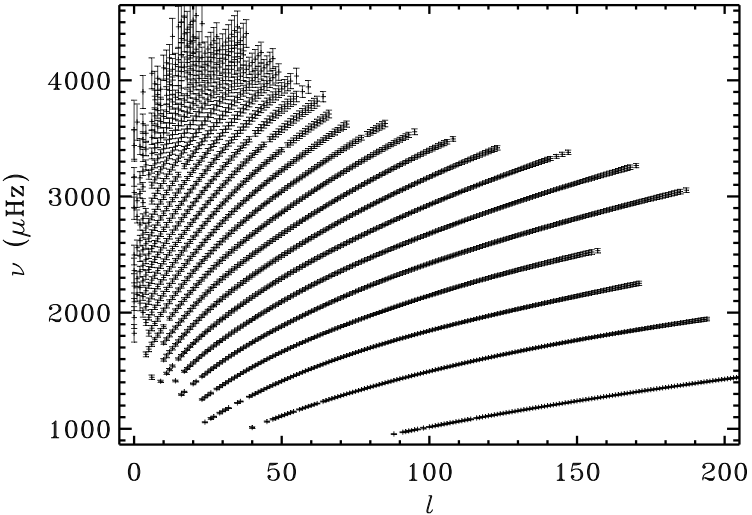
\includegraphics[keepaspectratio,width=0.95\textwidth]{midlmodes}
%\caption{I picchi della densit\'a spettrale si dispongono su creste in cui \'e concentrata la potenza in accordo al modello. Determinata usando i primi 144 giorni di osservazione di MDI con $l\leq300$. Da \cite{chr02helioseismology}.}\label{fig:midlmodes}
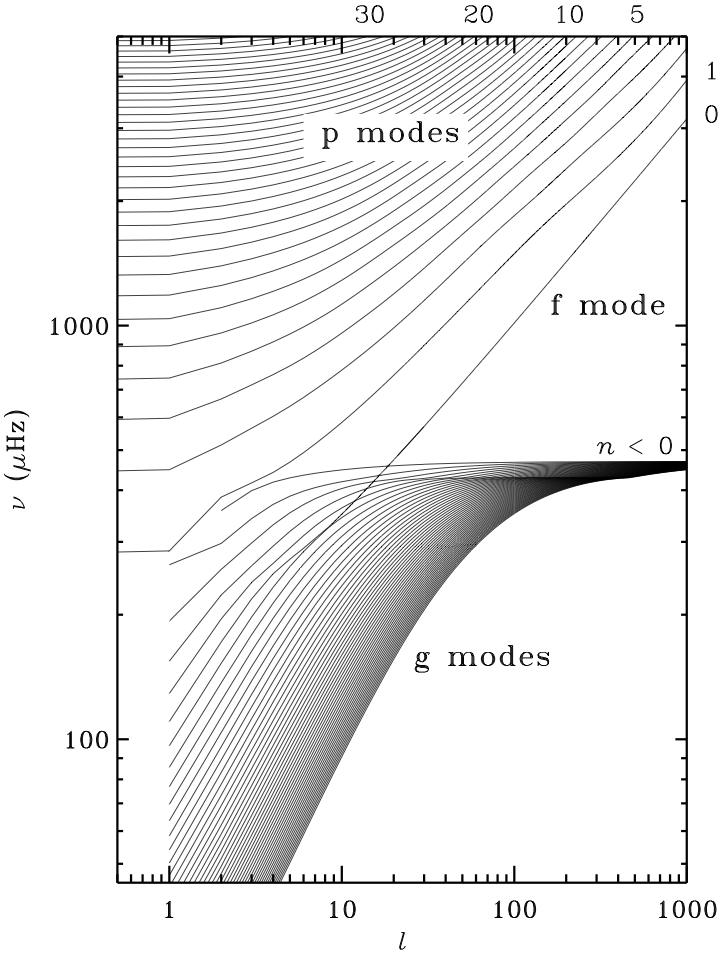
\includegraphics[keepaspectratio,width=0.9\textwidth]{nrmodesLAWE}
\caption{Da \cite{chr02helioseismology}.}%\label{fig:nrmodesLAWE}
\end{figure}

\end{column}

\end{columns}

\end{frame}

\begin{wordonframe}{Spettro dei modi: modi p, modi g, modi f}

La figura mostra lo spettro delle frequenze discrete per cui il sistema dei modi ha soluzione in funzione del grado angolare l. I modi con stesso ordine radiale sono uniti da una linea: nella parte ad alte frequenze abbiamo i modi p, di natura acustica, nella parte a basse frequenze modi g, che sono onde di gravit\'a, e modi f, modi di superficie ($\div{\vec{\xi}}\approx0$, $\omega^2=gk_h$). 

L'energia cinetica del modo $(n,l)$ mediata su un periodo \'e la media temporale dell'integrale della densit\'a di energia sul volume solare: \'e utile introdurre l'inerzia normalizzata all'ampiezza superficiale.

\end{wordonframe}

\begin{frame}{Osservazione delle oscillazioni della fotosfera}

\begin{figure}[!ht]

%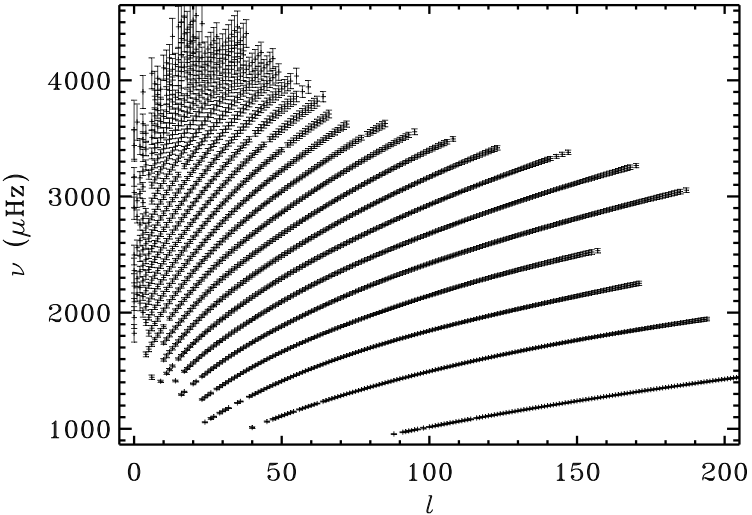
\includegraphics[keepaspectratio,width=0.95\textwidth]{midlmodes}
%\caption{I picchi della densit\'a spettrale si dispongono su creste in cui \'e concentrata la potenza in accordo al modello. Determinata usando i primi 144 giorni di osservazione di MDI con $l\leq300$. Da \cite{chr02helioseismology}.}\label{fig:midlmodes}

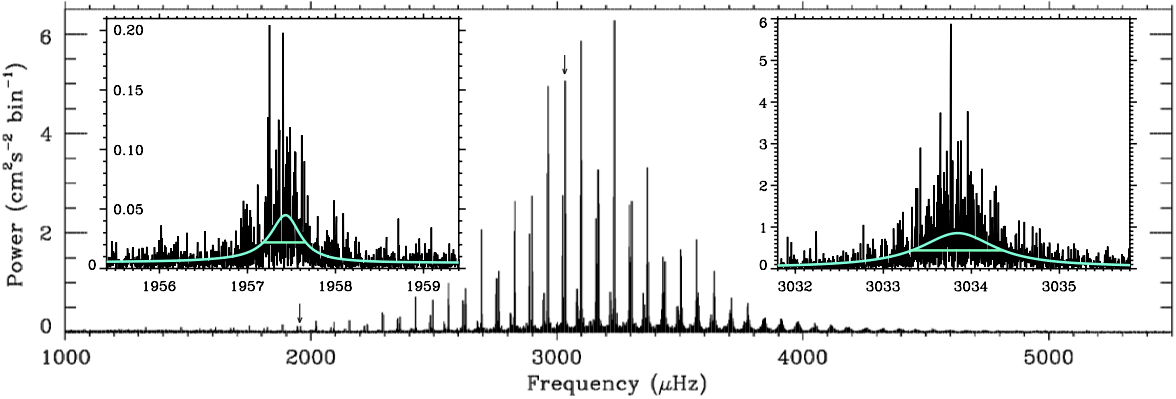
\includegraphics[keepaspectratio,width=0.95\textwidth]{PSD}
\caption{Da \cite{houdek2006stochastic}.}\label{fig:PSD}

\end{figure}

\begin{align*}
&I_{nl}[\TtwoDy{t}{A_{nl}}+\Gamma_{nl}\TDy{t}{A_{nl}}+\omega_{nl}^2A_{nl}]=f(t)\\
&P(\omega)\propto P_LP_f=\frac{\midfrac{\Gamma_{nl}}{2\pi}}{(\omega-\omega_{nl})^2+\midfrac{\Gamma_{nl}}{4}}P_f\\
&P_x(\nu)=\sum_i\frac{AB_i\midfrac{\Gamma^2}{4}}{(\nu-\nu_0-\Delta\nu_i)^2+\midfrac{\Gamma^2}{4}}+P_n(\nu)\\
&\exv{V_{nl}^2}=I_{nl}\frac{1}{T_{obs}}\int_{-\infty}^{\infty}|V_{nl}(\nu)|^2\,d\nu\propto I_{nl}\Gamma_{nl}A_{nl}
\end{align*}


\end{frame}

\begin{wordonframe}{Forma dei picchi nella PSD}

Lo studio delle oscillazioni solari come disciplina \'e l'eliosismologia. L'eliosismologia nasce all'inizio degli anni ''60 quando Leighton e collaboratori osservarono un comportamento oscillatorio nell'atmosfera solare con periodo attorno ai 5 minuti.

Questo comportamento \'e dovuto alla sovrapposizione di onde acustiche instappolate in cavit\'a risonanti a diversa profondit\'a a seconda delle grandezze caratteristiche orizzontale. Le frequenze dei modi sono determinate dalla velocit\'a del suono in queste regioni imponendo che  la cavit\'a contenga radialmente un numero semi-intero di lunghezze d'onda. \'E possibile quindi determinare il profilo radiale della velocit\'a del suono dalle frequenze dei modi osservate.


(modi basso l: N=13, n=21)

Le frequenze dei modi sono determinate principalmente misurando lo spostamento doppler di opportune righe di assorbimento in atmosfera ($Ca \lambda=6439 A 129 Km$, $K: 7699 A, 250Km$, $Ni I: 6708 A,300 Km$, $Na D1/D2: 5690 A, 500 Km$). Per identificare modi con $l>2$ \'e necessaria risolouzione spaziale e la proiezione di un'opportuna maschera $W_{l_0m_0}$ isoler\'a il modo con dipendenza spaziale descritta da $Y_{l_0m_0}$. La serie temporale del segnale doppler viene analizzata in termini di componenti armoniche. Le frequenze sono quindi determinate fittando i picchi dello spettro secondo una forma lorentziana  giustificata assumendo che l'ampiezza superficiale dei modi obbedisca all'equazione del moto di un'oscillatore armonico smorzato di frequenza naturale data dalla frequenza del modo e forzante stocastica.

La PSD $P_T(\nu)=\frac{1}{T_{obs}}|X_T(\nu)|^2$ contiene oltre al picco principale (lorentziano) picchi parassiti dovuti a gap nella serie temporale e il contributo del rumore solare.

\end{wordonframe}

\begin{frame}{Modello dell'ampiezza superficiale delle oscillazioni}

\begin{columns}

\begin{column}{0.4\textwidth}

\begin{figure}[!ht]
\centering
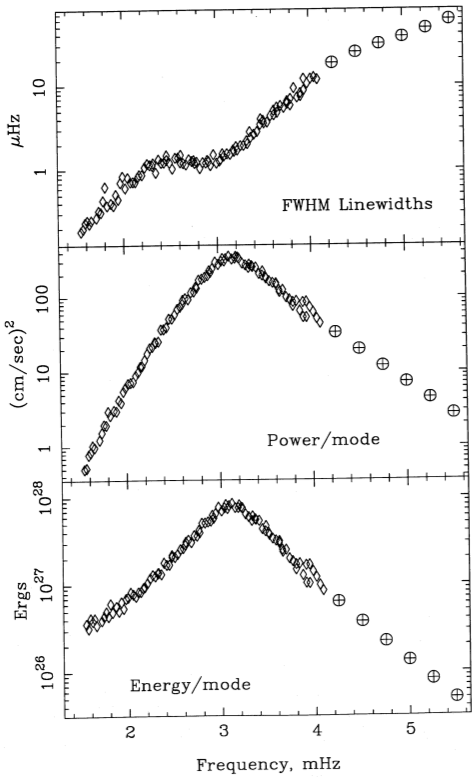
\includegraphics[keepaspectratio,width=0.85\textwidth]{modespheomenology}
\caption{Da \cite{libbrecht1988solar}.}\label{fig:Powerspectraldensity}
\end{figure}

\end{column}

\begin{column}{0.6\textwidth}

\begin{align*}
%&I_{nl}[\TtwoDy{t}{A_{nl}}+\Gamma_{nl}\TDy{t}{A_{nl}}+\omega_0^2A_{nl}]=f(t)\\
%&P(\omega)\propto P_LP_f=\frac{\midfrac{\Gamma_{nl}}{2\pi}}{(\omega-\omega_{nl})^2+\midfrac{\Gamma_{nl}}{4}}P_f\\
&\TDy{t}{E_{nl}}+\Gamma_{nl}E_{nl}=\exv{\dvec{\xi}_{nl}\cdot\vec{F}}\\
&\bar{E}_{nl}=I_{nl}\exv{V_{nl}^2}=I_{nl}\frac{1}{T_{obs}}\int_{-\infty}^{\infty}|V_{nl}(\nu)|^2\,d\nu\propto I_{nl}\Gamma_{nl}A_{nl}\\
&\bar{E}_{nl}=\frac{\exv{\dvec{\xi}_{nl}\cdot\vec{F}}}{\Gamma_{nl}}
\end{align*}
%dove $\exv{\dvec{\xi}_{nl}\cdot\vec{F}}$ \'e il lavoro della forzante mediato su un periodo.

\end{column}

\end{columns}

\end{frame}

\begin{wordonframe}{Ampiezza delle oscillazioni}

L'energia dell'oscillatore varia su tempi scala proporzionali a $\invers{\Gamma}_{nl}$ attorno al valor medio $\bar{E}_{nl}$:

\end{wordonframe}


\begin{frame}{Relazione di dispersione per onde gravo-acustiche: cavit\'a risonanti.}


\begin{align*}
%&\omega_A=\frac{c_s}{2\densityscale{}}\sqrt{1-2\TDy{r}{\densityscale{}}}\propto T\expy{-\frac{1}{2}}\\%\label{eq:acusticcutoff} \intxt{quindi ottengo la relazione di dispersione:}
%&\vec{\xi}\propto\exp{i\scap{k}{r}}\\
&\TtwoDy{r}{\xi_r}=\frac{\omega^2}{c_s^2}(1-\frac{N^2}{\omega^2})(\frac{S_l^2}{\omega^2}-1)\xi_r=-k_r^2\xi_r
\end{align*}

\begin{columns}

\begin{column}{0.4\textwidth}
Onde acustiche:\[k_r^2=\frac{\omega^2}{c_s^2}(\frac{S_l^2}{\omega^2}-1)\]
Raggio di inversione del moto:\[\frac{k_h^2}{\omega^2}=c_s^2\]
Onde di gravit\'a:\[k_r^2=\frac{S_l^2}{c_s^2}(\frac{N^2}{\omega^2}-1)\]

\end{column}

\begin{column}{0.6\textwidth}

\begin{figure}[!ht]
\centering
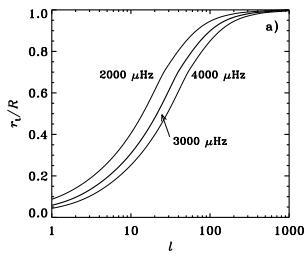
\includegraphics[keepaspectratio,angle=0,width=0.9\textwidth]{plowertp}
\caption{Da \cite{dal03notes}.}\label{fig:plowertp}
\end{figure}

\end{column}

\end{columns}

\end{frame}

\begin{wordonframe}{Relazione di dispersione e frequenze critiche}

\end{wordonframe}

\begin{frame}{Condizione di risonanza radiale}


\begin{figure}[!ht]
\centering
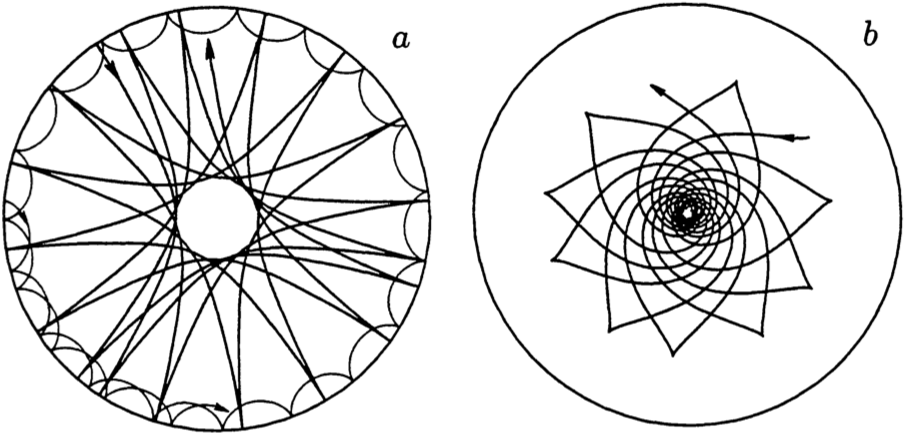
\includegraphics[keepaspectratio,width=0.6\textwidth]{raypath-gp}
\caption{Da\cite{gou91seismic}.}
\end{figure}

\begin{align*}
%&(n+\alpha)\pi\approx\int_{r_t}^Rk_r\,dr\\
&(n+\alpha)\pi\approx\int_{r_t}^R\frac{\omega}{c_s}\sqrt{1-\frac{S_l^2}{\omega^2}}\,dr
\quad
\frac{(n+\alpha_g)\pi}{L}\approx\int_{r_1}^{r_2}(\frac{N^2}{\omega^2}-1)\expy{\frac{1}{2}}\,d\ln{r}
\end{align*}

\end{frame}

\begin{wordonframe}{Condizione di risonanza radiale}

La condizione di risonanza radiale \'e nota come legge di Duvall per modi p

\end{wordonframe}

\begin{frame}{Effetti delle regioni superficiali sulle frequenze dei modi}

\begin{columns}

\begin{column}{0.5\textwidth}

\begin{figure}
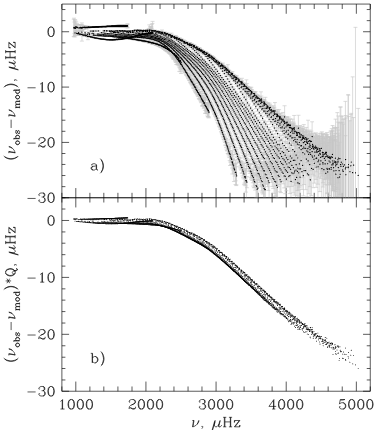
\includegraphics[keepaspectratio,width=0.7\textwidth]{domega}
\captionof{figure}{Da \cite{rhodesmeasurements}.}
\end{figure}

\end{column}

\begin{column}{0.5\textwidth}
%\begin{figure}[!ht]
%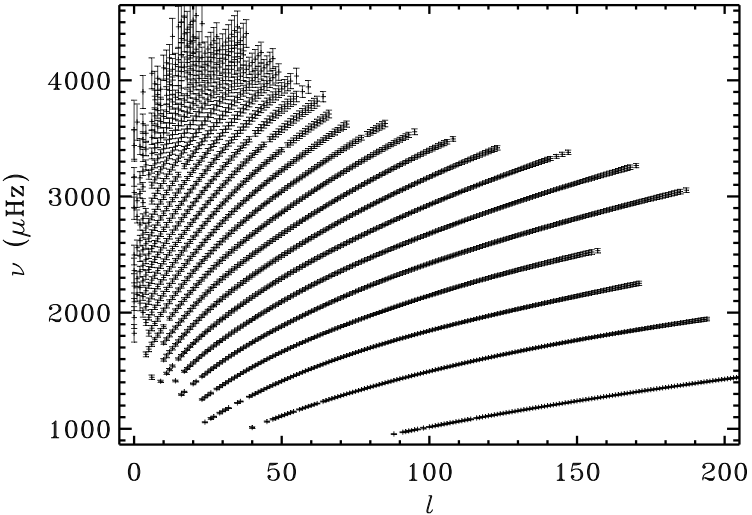
\includegraphics[keepaspectratio,width=0.95\textwidth]{midlmodes}
%\caption{I picchi della densit\'a spettrale si dispongono su creste in cui \'e concentrata la potenza in accordo al modello. Determinata usando i primi 144 giorni di osservazione di MDI con $l\leq300$. Da \cite{chr02helioseismology}.}\label{fig:midlmodes}
%
\begin{align*}
&\omega_A=\frac{c_s}{2\densityscale{}}\sqrt{1-2\TDy{r}{\densityscale{}}}\propto T\expy{-\frac{1}{2}}
\end{align*}


%\end{figure}
\end{column}

\end{columns}

\end{frame}

\begin{wordonframe}{Effetti delle regioni superficiali sulle frequenze dei modi}

Contributo non-adiabatico ($\alpha(\omega)$): differenze dovute a effetti non adiabatici in superficie maggiori per l maggiori perche confinati in guscio sottile e maggiori ad alte frequenze perch\'e punto di inversione pi\'u in alto.

\end{wordonframe}
%$\omega_c=\frac{c_s}{2\densityscale{}}\sqrt{1-2\TDy{r}{\densityscale{}}}\propto T\expy{-\frac{1}{2}}$
%$S_l^2=\frac{l(l+1)c_s^2}{r^2}$.
%$N^2=g(\frac{1}{\Gamma_1P}\TDy{r}{P}-\frac{1}{\rho}\TDy{r}{\rho})=g(\frac{1}{\densityscale{}}-\frac{g}{c_s^2})$

\begin{comment}

\begin{frame}{Espressioni asintotiche per le frequenze}

\begin{columns}

\begin{column}{0.5\textwidth}

\begin{block}{Modi p con l grande}
\begin{equation*}
\omega_{nl}^2=\frac{2}{\mu_p}\frac{g}{\rsun{}}(n+\alpha)L
\end{equation*}
\end{block}

\end{column}

\begin{column}{0.5\textwidth}

\begin{block}{Modi p con l piccolo}

\begin{equation*}
\nu_{nl}=\frac{\omega_{nl}}{2\pi}\approx(n+\frac{l}{2}+\frac{1}{4}+\alpha)\Delta\nu*\label{eq:freqequi}
\end{equation*}
\[\Delta\nu=[2\int_0^R\frac{dr}{c}]\expy{-1}\approx\SI{136}{\micro\hertz}\]

\end{block}

\end{column}

\end{columns}

\begin{block}{Modi g di alto n e basso l}

\begin{equation*}
\omega=\frac{L\int_{r_1}^{r_2}N\frac{dr}{r}}{\pi(n+\frac{l}{2}+\alpha_g)}
\end{equation*}
 $\lim_{n\to\infty}{\alpha_g}\approx-\midfrac{1}{6}$

\end{block}

\end{frame}

\begin{wordonframe}{Espressioni asintotiche per le frequenze}

\end{wordonframe}

\end{comment}



\part{Tecniche e risultati di inversione}\label{part:inverseproblem}

\frame{\partpage}


\begin{frame}{Inversione assoluta}


\begin{equation*}
c_s^2=\Gamma_1\frac{P}{\rho}
\end{equation*}

%\begin{columns}
%\begin{column}{0.6\textwidth}
\begin{figure}[!ht]
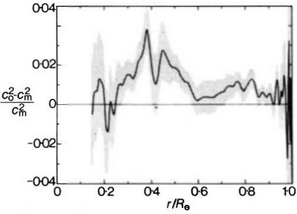
\includegraphics[height=0.45\textheight,keepaspectratio]{dsoundspeedduvall} 

%\end{column}
%\begin{column}{0.4\textwidth}
\captionof{figure}{%Differenza relativa del profilo di $c_s$ (determinata invertendo \eqref{eq:analinversionc}) per frequenze dei modi calcolate con MSS e osservate. La differenza relativa \'e minore del $5\%$.
Da \cite{christensen1985speed}.}
\label{dsoundduvall}
\end{figure}
%\end{column}
%\end{columns}

\end{frame}

\begin{wordonframe}{Inversione legge di DUvall}

Il profilo radiale della velocit\'a del suono risultante  mostra la validit\'a del modello solare (detto standard per contrasto con i modelli pensati per risolvere il problema dei neutrini solari.)

(Errore sistematico dovuto alle approssimazione di Cowling intorno al $2.5\%$)

Il modello MSS si basa su leggi di conservazione, valide per qualsiasi stella: le prime 3 equazioni usate per determinare la struttura stellare ...

\end{wordonframe}

%\section{Principio variazionale}

\begin{frame}{Effetto di perturbazioni nell'equazione del moto sulle frequenze}

\begin{block}{Problema agli autovalori hermitiano}

\begin{align*}%\label{eq:EOMrhoc}%Unno89
&L(\vec{\xi})=\frac{1}{\rho_0}\nabla p'-\vec{g}'-\frac{\rho'}{\rho_0}\vec{g}_0\\
&\rho_0L(\xi)=\nabla(c_s^2\rho\scap{\nabla}{\xi}+\nabla P\cdot\vec{\xi})-\vec{g}_0\nabla\cdot(\rho_0\vec{\xi})-G\rho_0\nabla(\int_V\frac{\nabla\cdot(\rho_0\vec{\xi})\,d^3r'}{|\vec{r}-\vec{r}'|})\\
&L(\xi)=-\omega^2\xi
\end{align*}

\end{block}

\begin{block}{Variazioni nell'equazione del moto perturbato}

\begin{equation*}
(L+\Lvar{L})(\xi+\Lvar{\xi})=-(\omega+\Lvar{\omega})^2(\xi+\Lvar{\xi})%&\label{eq:EMvar}
\end{equation*}

\end{block}

\begin{block}{Variazioni nelle frequenze}

\[\frac{\Lvar{\omega}}{\omega}=-\frac{\int_V\rho\vec{\xi}\Lvar{L}\vec{\xi}\,d^3x}{2\omega^2\int_V\rho\scap{\xi}{\xi}d^3x}\]

\end{block}

\end{frame}

\begin{wordonframe}{Principio variazionale}

Definisco l'operatore lineare L riscrivendo l'equazione del moto perturbato in termini di $\vec{\xi}$ e delle grandezze di equilibrio. 

Chandrasekhar ha dimostrato che L definisce un problema agli autovalori hermitiano per condizioni alla superfice stellare di pressione e densit\'a nulle.

Considero gli effetti di una variazione piccola di L, cio\'e una variazione dell'equazione del moto perturbato, $\delta L$ sulle frequenze dei modi. Tengo i termini lineari nelle perturbazioni e data la stazionariet\'a di $\omega$ rispetto a $\xi$ il termine $L\delta \xi$ \'e nullo. Moltiplicando per $\xi*$  e integrando sul volume stellare ottengo l'espressione per la variazione nelle frequenze dei modi in funzione della variazione dell'equazione del moto perturbato.

\end{wordonframe}

\begin{frame}{Variazione nei modi per variazione in struttura, equazione di stato e composizione}

\begin{block}{Inversione per $(c^2,\rho)$}

\begin{equation*}
\frac{\delta\omega_{nl}}{\omega_{nl}}=\int_0^R[K^{nl}_{c^2,\rho}(r)\frac{\delta_rc^2}{c^2}(r)+K^{nl}_{\rho,c^2}(r)\frac{\delta_r\rho}{\rho}(r)]\,dr+I_{nl}\expy{-1}F_{Surf}
\end{equation*}

\end{block}

\begin{block}{Inversione per $(u,Y)$}

\begin{equation*}
\frac{\delta\omega_{nl}}{\omega_{nl}}=\int_0^RK^{nl}_{u,Y}(r)\frac{\delta_ru}{u}(r)\,dr+\int K^{nl}_{Y,u}(r)\delta_rY\,dr+I_{nl}\expy{-1}F_{Surf}
\end{equation*}

\end{block}

\end{frame}

\begin{wordonframe}{Variazioni delle grandezze d'equilibrio $(c^2,\rho)$ e $(u,Y)$}

Considero variazioni nel profilo radiale di $(c^2,\rho)$: posso esprimere la variazione nelle frequenze dei modi usando il principio variazionale in termini delle variazioni in densit\'a e pressione tramite le funzioni kernel dipendenti dalle autofunzioni dei modi.

Analogamente  esprimo le differenze nelle frequenze dei modi in termini di variazioni al profilo radiale di $(u,Y)$ ma devo esplicitare la dipendenza di $\Gamma_1$ da Y usando l'equazione di stato.

\end{wordonframe}

\begin{frame}{Tecniche d'inversione}

\begin{block}{RLS}

I parametri sono determinati minimizzando:
\begin{equation*}
Y=\sum_{\alpha=1}^N(\frac{\delta\omega_{obs}-\delta\omega_{fit}}{\sigma})^2_{\alpha}+\alpha N\int_0^1(x\TDof{x}\frac{\Delta f}{f})^2\,dx
\end{equation*}

\end{block}

\begin{block}{Subtractive Optimally Localized Averaging.}

\begin{equation*}
\sum_ic_i(r_0)\frac{\delta\omega_i}{\omega_i}=\int_0^R\sum_ic_i(r_0)K^i(r)\frac{\delta f(r)}{f(r)}\,dr=\exv{\frac{\delta f(r_0)}{f(r_0)}}
\end{equation*}

I coefficienti $c_i(r_0)$ sono determina minimizzando la funzione
\begin{equation*}
\int_0^R[\mathcal{K}(r_0,r)-\mathcal{T}(r_0,r)]^2\,dr+\mu\sum_{ij}E_{ij}c_i(r_0)c_j(r_0)
\end{equation*}

\end{block}

\end{frame}

\begin{wordonframe}{Tecniche d'inversione}

Usando la tecnica del minimo $\chi^2$ regolarizzato si parametrizza la funzione incognita $\frac{\delta f}{f}$, tramite funzioni di base opportune, determinata minimizzando:

N indica il numero totale di modi $\alpha$, $N_p$ il numero di parametri da determinare, $\Delta\omega_{fit}$, ricavato tramite eq:variational, contiene la funzione incognita; il secondo addendo del lato destro di eq:minimizerls \'e introdotto per ridurre oscillazioni indesiderate nel risultato dell'inverisone con $\alpha$ parametro di regolarizzazione.

Determino dei coefficienti $c_i(r_0)$ tali che \[\sum c_i(r_0)\frac{\delta\omega_i}{\omega_i}\] fornisca una media del valore di $\frac{\delta f(r)}{f(r)}$ in $r=r_0$:

La larghezza finita di $\mathcal{K}(r_0,r)$ determina il valor medio di $\frac{\delta f}{f}$ in intorno di $r_0$ e ci\'o causa una differenza sistematica  dal valore effettivo in $r_0$: per $c_s$ l'errore \'e minore del $0.03\%$ e le regioni pi\'u afflitte sono la base della zona convettiva, per la rapida variazione di $\frac{\delta c_s}{c_s}$ e la regione centrale, per il ridotto numero di modi che penetrano in questar zona.

Illustro la tecnica SOLA per determinare $\frac{\delta_rc^2}{c^2}$: si formano delle combinazioni lineari di $\frac{\Lvar{\omega_i}}{\omega_i}$ pesate da coefficienti $c_i(r_0)$ tali che $\frac{\Lvar{c^2}}{c^2}$ sia centrato attorno $r_0$ e che gli altri termini in \eqref{eq:invstructure} siano soppressi, queste compongo un averaging kernel $\mathcal{K}_{c^2,\rho}(r_0,r)=\sum_ic_i(r_0)K_{c^2,\rho}^i(r)$, con $\int_0^R\mathcal{K}(r_0,r)\,dr=1$.


Determino i coefficienti minimizzando l'espressione
\begin{equation}
\int_0^R[\mathcal{K}_{c^2,\rho}(r_0,r)-\mathcal{T}(r_0,r)]^2\,dr+\beta\int_0^R\mathcal{L}_{\rho,c^2}(r_0,r)\,dr+\mu\sum_i\sigma_ic_i(r_0)c_j(r_0)
\end{equation}
dove il kernel cross-term
\begin{equation}
\mathcal{L}_{\rho,c^2}(r_0,r)=\sum_ic_i(r_0)K_{\rho,c^2}^i(r)
\end{equation}
controlla i contributi indesiderati di $\frac{\delta_r\rho}{\rho}$.

\end{wordonframe}

\begin{frame}{Accuratezza posizione base zona convettiva e abbondanza elio}

\begin{table}[!ht]%{r}{0.7\textwidth}

\pgfplotstabletypeset[
math/.style={%
        preproc cell content/.append style={/pgfplots/table/@cell content/.add={$}{$}},
    },
every head row/.style={
 before row={\toprule
 %&\multicolumn{4}{c|}{Primordiale}
 },
 every last row/.style={after row=\bottomrule},
 after row={\midrule}
},
every last row/.style={after row=\bottomrule},
every first column/.style={column type/.add={|}{}},
every last column/.style={column type/.add={}{|}},
%columns/0/.style = {column type/.add={|}{}},
display columns/0/.style={column name={Composizione}},
display columns/1/.style={column name={$Z/X$}},
display columns/2/.style={column name={$R_{CZ}$}},
display columns/3/.style={column name={$Y_{CZ}$}},
display columns/4/.style={column name={$Y_0$}},
create on use/comp/.style={create col/set list={
inversione,GS98,AGS05,AGSS09,C+11}},
columns/comp/.style = {column type/.add={|}{}},
columns/comp/.style={string type},
columns/ZX/.style={string type},
columns/ZX/.append style={math},
columns/RCZ/.style={string type},
columns/RCZ/.append style={math},
columns/YCZ/.style={string type},
columns/YCZ/.append style={math},
columns/Y0/.style={string type},
columns/Y0/.append style={math},
columns={comp,ZX,RCZ,YCZ,Y0},
%/pgf/number format/precision=4
     ]{CZvsZ.txt} %%%
     \caption{Da \cite{basu2016global}.}
\label{tab:CZZvar}
\end{table}

\end{frame}

\begin{wordonframe}{Accuratezza posizione base zona convettiva e abbondanza elio}

Confronto le caratteristiche della zona convettiva ricavati tramite inversione e  ricavate tramite modelli con diversa composizione.

I modelli con una minore metallicit\'a hanno una opacit\'a minore nella zona radiativa e quindi un minore gradiente termico a parit\'a di flusso (temperatura centrale minore).

Le differenze quadratiche medie nel profilo della velocit\'a del suono sono  correlate con corretta predizione della posizione della zona convettiva: nel caso non si verifiche il modello non riproduce correttamente il gradiente termico ...

\end{wordonframe}

\begin{frame}{Accuratezza profilo radiale della velocit\'a del suono}

\begin{figure}[!ht]%{r}{0.5\textwidth}
        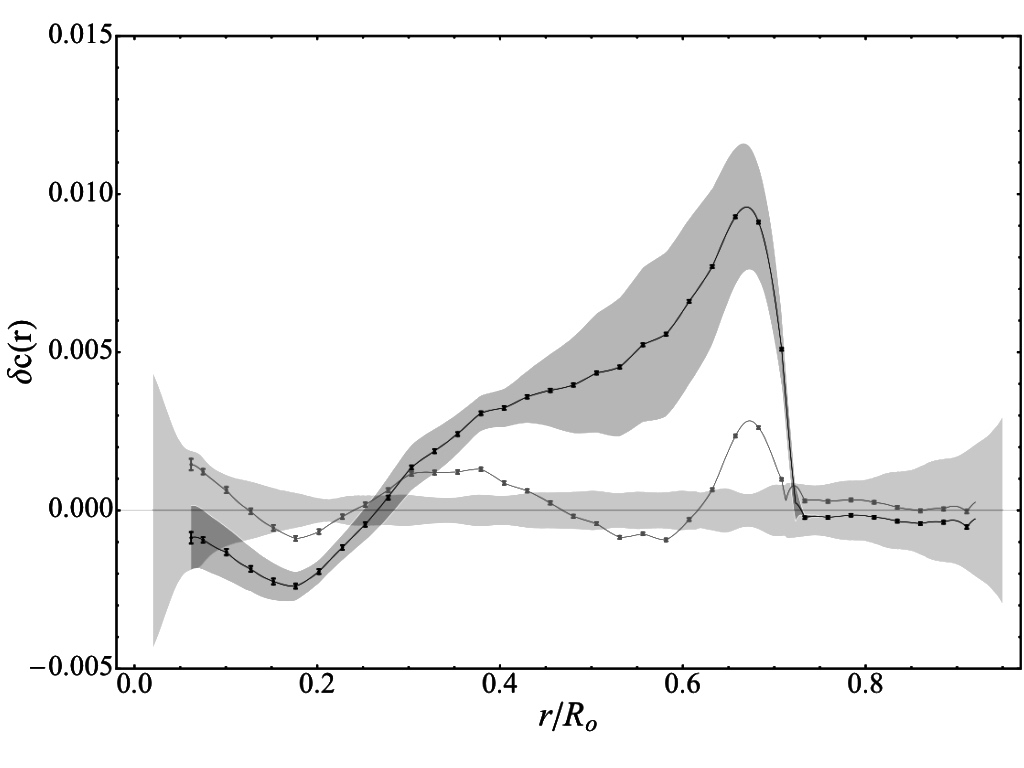
\includegraphics[width=0.8\textwidth,keepaspectratio]{deltacwu}
        \caption{Da \cite{villante2014chemical}.}\label{fig:deltacwu}
\end{figure}

\end{frame}

\begin{wordonframe}{Accuratezza profilo radiale della velocit\'a del suono}

Le differenze quadratiche medie nel profilo della velocit\'a del suono sono  correlate con corretta predizione della posizione della zona convettiva: nel caso non si verifiche il modello non riproduce correttamente il gradiente termico ...

Questa figura rappresenta le differenze nel profilo radiale della velocit\'a del suono risultanti dall'inversione delle frequenze osservate per un modello con composizione $\midfrac{Z}{X}=0.023$ (GS98), linea rossa, e uno con $\midfrac{Z}{X}=0.018$ (AGSS09), linea nera.

La banda rossa intorno allo zero che rappresenta il profilo effettivo della velocit\'a del suono nel Sole indica l'errore dovuto alle tecniche di inversione, alle incertezze sulle frequenze e alla residua dipendenza dell'inversione dal modello solare.

\end{wordonframe}

\section{Appendix}


\begin{frame}{Modello plasma solare}

\begin{block}{Processi che contribuiscono all'opacit\'a}

Transizioni tra stati elettronici (BB).

Ionizzazione (BF).

Brehmstrahlung inverso (FF).

Scattering di elettroni (S).

\end{block}

\vfill

\begin{block}{Opacit\'a media di Rosseland}

\vfill

\begin{equation*}
\frac{1}{\kappa}=\invers{(4aT^3)}\int_0^{+\infty}\PDy{T}{B_{\nu}(T)}\frac{1}{\kappa_{a}(\nu)(1-\exp{-\midfrac{h\nu}{KT}})+\kappa_s(\nu)}\,d\nu
\end{equation*}

\end{block}

\vfill

\end{frame}

\begin{wordonframe}{Interazioni radiazione-materia}

L'interazione radiazione-materia determina il gradiente termico della regione radiativa e nel caso solare la posizione della base della zona convettiva. L'opacit\'a \'e dovuta ai processi di assorbimento e scattering dei fotoni e dipende dal numero dalla densit\'a di particelle che danno luogo a un determinato fenomeno di assorbimento o scattering e dalla sezione d'urto per singola particella.

L'opacit\'a media per grammo () \'e determinata mediando l'opacit\'a a data lunghezza d'onda rispetto a $\PDy{T}{B_{\nu}(T)}$. L'opacit\'a a data frequenza \'e somma dei contributi da parte dei processi di assorbimento (bb, bf, ff) e scattering.

C'\'e un ulteriore correzione che tiene conto della frazione di emissione spontanea su totale.

\end{wordonframe}

\begin{frame}{Catena PP}

\begin{block}{Contributo della fusione di nuclei $(i,j)$ alla produzione di energia per grammo}

\begin{align*}
&\epsilon_{ij}=\frac{1}{1+\delta_{ij}}Q_{ij}\frac{\rho N_A^2X_iX_j}{{A_iA_j}}\exv{\sigma v}_{ij}%\label{eq:energyrate}
\end{align*}
\end{block}


\begin{columns}

\begin{column}{0.65\textwidth}

\begin{block}{Fusione idrogeno in elio: catena PP}

\setmuskip{\thinmuskip}{0mu}\setmuskip{\medmuskip}{0mu}
\tikzset{->-/.style={decoration={
  markings,
  mark=at position .5 with {\arrow{>}}},postaction={decorate}},
-->/.style={decoration={
  markings,
  mark=at position .8 with {\arrow{>}}},postaction={decorate}},
box/.style={%
%draw,
minimum width=25mm,%
    minimum height=6mm,%
    align=center}
}

\centering
\begin{tikzpicture}

\begin{scope}[scale=0.6,transform shape]
\node[box] (pp) at (0,0) {$\Pproton{+}\Pproton{\to}\cel{H}{2}{}{}{+}\Pnue{+}\APelectron$};%%pp
\node[box,right=2cm of pp]  (pep) {$\Pproton{+}\Pproton{+}\Pelectron{\to}\cel{H}{2}{}{}+\Pnue$};%%pep
\coordinate[below=0.3cm of pp] (bpp);
\node[left] at (bpp) {$99.76\%$};
\coordinate[below=0.3cm of pep] (bpep);
\node[right] at (bpep) {$0.24\%$};

\coordinate[] (ttriton) at ($(bpp)!0.5!(bpep)$);
\draw[->-] (pp)--(bpp)--(ttriton);
\draw[->-] (pep)--(bpep)--(ttriton);
\node[box,below=0.3cm of ttriton] (triton) {$\Pproton+\cel{H}{2}{}{}\to\cel{He}{3}{}{}+\Pphoton$};%%triton
\coordinate[below=0.3cm of triton] (btriton);
\draw[-->] (ttriton)--(triton.north);
\draw[->-] (triton.south)--(btriton.north);
\coordinate[left=2.5cm of btriton] (tpp1);
\node[left] at (tpp1) {$83.3\%$};
\coordinate[right=2.0cm of btriton] (tberillium7);
\node[above] at (tberillium7) {$16.7\%$};
\coordinate[right=6.5cm of btriton] (thep);
\node[right] at (thep) {$\num{2e-5}\%$};

\draw[] (btriton)--(tpp1);
\draw[] (btriton)--(tberillium7);
\draw[] (tberillium7)--(thep);
\node[box,below=0.5cm of tpp1,label={[xshift=0.1cm, yshift=-1.5cm]PPI}]  (pp1) {$\cel{He}{3}{}{}+\cel{He}{3}{}{}\to\cel{He}{4}{}{}+2\Pproton$};%%pp1
\node[box,below=0.5cm of tberillium7]  (berillium7) {$\cel{He}{3}{}{}+\cel{He}{4}{}{}\to\cel{Be}{7}{}{}+\Pphoton$};%%berillium7
\node[box,below=0.5cm of thep,label={[xshift=-0.1cm, yshift=-1.5cm]HEP}]  (hep) {$\cel{He}{3}{}{}+\Pproton\to\cel{He}{4}{}{}+\APelectron+\Pnue$};%%hep

\draw[->-] (tpp1)--(pp1.north);
\draw[->-] (tberillium7)--(berillium7.north);
\draw[-->] (thep)--(hep.north);

\coordinate[below=0.3cm of berillium7] (bberillium7);
\coordinate[left=1.5cm of bberillium7] (tlithium7);
\node[left] at (tlithium7) {$99.88\%$};
\coordinate[right=2.0cm of bberillium7] (tboron8);
\node[right] at (tboron8) {$0.12\%$};

\node[box,below=0.5cm of tlithium7]  (li7) {$\cel{Be}{7}{}{}+\Pelectron\to\cel{Li}{7}{}{}+\Pnue$};%%Li7
\node[box,below=0.5cm of li7,label={[xshift=0.1cm, yshift=-1.5cm]PPII}] (pp2) {$\cel{Li}{7}{}{}+\Pproton\to2\cel{He}{4}{}{}$};%% PP2

\node[box,below=0.5cm of tboron8]  (b8) {$\cel{Be}{7}{}{}+\Pproton\to\cel{B}{8}{}{}+\Pphoton$};%%B8
\node[box,below=0.25cm of b8]  (be7) {$\cel{B}{8}{}{}\to\cel{Be}{8}{}{}^*+\APelectron+\Pnue$};%%Be8*
\node[box,below=0.25cm of be7,label={[xshift=0.1cm, yshift=-1.5cm]PPIII}]  (pp3) {$\cel{Be}{8}{}{}^*\to2\cel{He}{4}{}{}$};%%pp3

\draw[->-] (berillium7.south)--(bberillium7);
\draw[] (bberillium7)--(tlithium7);
\draw[] (bberillium7)--(tboron8);

\draw[->-] (tlithium7)--(li7.north);
\draw[->-] (li7.south)--(pp2.north);

\draw[->-] (tboron8.south)--(b8.north);
\draw[->-] (b8.south)--(be7.north);
\draw[->-] (be7.south)--(pp3.north);
\end{scope}

\node[] at (2,-4.5) {\parbox{0.8\textwidth}{\captionof{figure}{Da \cite{adelberger2011solar}.}}};

\end{tikzpicture}

\end{block}

\end{column}

\begin{column}{0.35\textwidth}

\begin{block}{Perdite in neutrini (Sole)}
\begin{tabular}{cc}
Ramo&$Q_{eff} (MeV)$\\
PP1&$26.2 (2\%)$\\
PP2&$25.66  (4\%)$\\
PP3 &$19.17 (28\%)$\\
\end{tabular}

\end{block}

\begin{block}{Tempo di vita}

{\small\begin{tabular}{cc}
&$\tau(\si{\year})$\\
$\cel{H}{1}{}{}(p,e^+\Pnue)\cel{D}{2}{}{}$&\num{8e9}\\
$\cel{D}{2}{}{}(p,\gamma)\cel{He}{3}{}{}$&\num{4.4e-8}\\
$\cel{He}{3}{}{}(\cel{He}{3}{}{},2p)\cel{He}{4}{}{}$&\num{2.4e5}\\
%$\cel{B}{8}{}{}\cel{Be}{8}{}{}^*\cel{He}{4}{}{}$&\num{3e-8}\\

\end{tabular}
}

\end{block}

\end{column}

\end{columns}

%\begin{block}{Tempi reazione e energia efficace prodotta}
%\begin{tabular}{c|c|}
%\hline
%Reazione & $t_r$ \\
%\hline
%$^1H+^1H\to^2H+\APelectron+\Pnue$ & $7*10^9\,yr$\\
%$^2H+^1H\to ^3He+\gamma$ & $4 s$\\
%$^3He+^3He\to^4He+2^1H$ & $4*10^5\,yr$\\
%\hline
%\end{tabular}
%\end{block}

\end{frame}

\begin{wordonframe}{Catena PP}

nella fase di sequenza principale la reazione efficace \'e la conversione di 4 nuclei di idrogeno in elio + 2 positroni e 2 neutrini.

Nel centro solare circa il $99\%$ della di $\epsilon$ \'e prodotto dalla catena PP.
Questa figura descrive le reazioni nucleari per condizioni del centro solare. 

\end{wordonframe}


% SOS
%\part{SSM (sos)}
%\begin{comment}
\section{Osservabili stellari/demo beamer}
\begin{frame}<1>[label=noinside]{Modello stellare}{Come indagare la fisica interna a una stella?}
\onslide<1->\begin{block}{Osservabili stellari:}
$L$, $M$, $R$, $T_e$, $(\frac{Z}{X})_{ph}$, $g_{ph}$.
\end{block}
\onslide<1->\begin{block}{Informazioni sulla struttura interna?} Condizione di equilibrio idrostatico
\end{block}
%Teorema Vogt-Russel: $X_i(r)$, $M$ \pause equilibrio (idrostatico/termico) determinano struttura stellare .
%\pause
\onslide<1->\begin{block}{Modello stellare: diagramma di \hr{}.}
\end{block}
\onslide<2->\begin{block}{Descrizione fisica interno stellare: parametri aggiuntivi}
Convezione, diffusione e sedimentazione elementi pesanti, equazione di stato, opacit\'a
\end{block}
\onslide<2->\begin{block}{Astrosismologia}
Restringo spazio parametri sistemi stellari lontani
\end{block}
\end{frame}
{ % all template changes are local to this group.
    \setbeamertemplate{navigation symbols}{}
    \begin{frame}[plain]{Diagramma di \hr{}}
        \begin{tikzpicture}[remember picture,overlay]
            \node[at=(current page.center)] {
                %\includegraphics[width=\paperwidth]{yourimage}
            };
        \end{tikzpicture}
     \end{frame}
}
\againframe<2>{noinside}
\begin{frame}{Pulsazioni stellari}{Modi Normali}
\begin{columns}
\begin{column}{0.5\textwidth}  %%<--- here
    \begin{center}
     %\includegraphics[width=0.5\textwidth]{image1}
     \end{center}
\end{column}
\begin{column}{0.5\textwidth}
\onslide<1-> \begin{block}{Stelle pulsanti}
Onde stazionarie: Pulsazione radiale/non radiale: .
\onslide<2-> meccanismo di eccitazione: solar-like pulsator, Cefeidi.
\onslide<3-> Modo fondamentale $\Pi\approx\tau_{dyn}=\sqrt{\frac{R^3}{GM}}\propto\overline{\rho}\expy{-\frac{1}{2}}$.
\onslide<4-> Modi di oscillazione\onslide<5-> - informazioni sull'interno stellare
\onslide<5-> Elio-sismologia: Modi $\Leftrightarrow$ Modelli solari
\onslide<5-> Astero-sismologia: Modi $\Leftrightarrow$ Spazio parametri modello stellare
\end{block}
\end{column}
\end{columns}
\end{frame}

\end{comment}

\section{Osservabili solari}

\begin{frame}{Dati osservativi}

\begin{block}{Et\'a, luminosit\'a, raggio solari}
\begin{tabular}{l|c}
\hline
$\agesun{}$&\SI[separate-uncertainty=true]{4.57\pm0.02e9}{\year}\\
\hline
$\rsun{}$&\SI{695658+-140}{\kilo\meter}\\
\hline
$G\msun$&\num{132712440018+-8}\SI{e9}{\cubic\meter\per\square\second}\\
\hline
$\lsun{}$&\SI{3.8275+-0.0014e33}{\erg\per\second}\\
\hline
\end{tabular}
%\caption[Osservabili solari principali.]{Osservabili solari principali. \cite{haberreiter2008solving}.}
\label{tab:sunO}
\end{block}

\begin{block}{Simmetria sferica}
Deviazioni da forma sferica trascurabili (campi magnetici, rotazione)
\end{block}

\end{frame}

\begin{frame}{Dati osservativi}

\begin{block}{Composizione chimica}
\begin{itemize}[noitemsep,topsep=0pt,parsep=0pt,partopsep=0pt]
\item Righe di assorbimento: attuale (non $Y_{ph}$)
\item Meteoriti CI: primordiale (refrattari)
\end{itemize}

\begin{table}[]

\pgfplotstabletypeset[
every head row/.style={
 before row={\toprule &\multicolumn{4}{c|}{Attuale}
 %&\multicolumn{4}{c|}{Primordiale}
 \\\midrule},
 every last row/.style={after row=\bottomrule},
 after row={\midrule}
},
every nth row={2}{before row=\midrule},every last row/.style={after row=\bottomrule},
every first column/.style={column type/.add={|}{}},
every last column/.style={column type/.add={}{|}},
columns/x/.style = {column type/.add={|}{}},
columns/xi/.style = {column type/.add={|}{}},
display columns/0/.style={column name={}},
display columns/1/.style={column name={$X$}},
display columns/2/.style={column name={$Y$}},
display columns/3/.style={column name={$Z$}},
display columns/4/.style={column name={$\frac{Z}{X}$}},
%display columns/5/.style={column name={$X$}},
%display columns/6/.style={column name={$Y$}},
%display columns/7/.style={column name={$Z$}},
%display columns/8/.style={column name={$\frac{Z}{X}$}},
create on use/authors/.style={create col/set list={
%Anders \& Grevesse (1989),Grevesse \& Noels (1993),
Grevesse et al. (1998),Lodders (2003),Asplund et al. (2005),Lodders et al. (2009),\cite{asplund2009chemical},\cite{caffau2011solar}}},
columns/authors/.style={string type},
columns={authors,x, y, z, zx
%,xi,yi,zi, zxi
},
/pgf/number format/precision=4
     ]{asplund.txt} %%%
\captionof{table}{Metallicit\'a attuale determinata da varii autori.}\label{tab:Zhistory}
\end{table}

\end{block}

\end{frame}


\section{Strutture autogravitanti in equilibrio}

\begin{frame}{Distribuzione di massa - Conservazione di massa e momento - tempo scala dinamico}

\begin{block}{Massa}

%\begin{align}
%&dm=4\pi r^2\rho \,dr-4\pi r^2\rho v\,dt\label{eq:massvar}\\
%\end{align}

\begin{equation}
\PDy{t}{\rho}+\nabla\cdot(\rho\vec{v})=0\label{eq:continuityeq}
\end{equation}

\begin{equation}
dm=4\pi r^2\rho \,dr\label{eq:massaguscio}
\end{equation}

\end{block}

\begin{block}{Momento}
\begin{align}
&\rho\TDy{t}{\vec{v}}=-\nabla P+\rho\vec{f}\label{eq:motion}\\
&\vec{g}=-\PDy{r}{\Phi}=-\frac{Gm(r)}{r^2}\hat{r}
\end{align}
\end{block}

\end{frame}

\begin{frame}{Equilibrio idrostatico: $\ddvec{r}=0$.}

\begin{align*}
\nabla P=\rho \vec{f}\Label{eq:idrosta} \TDy{r}{P}=-\frac{Gm(r)\rho(r)}{r^2}\Label{eq:fidroequilibrio}
\end{align*}


Per giustificare l'ipotesi di equilibrio idrostatico stimo i tempi caratteristici di evoluzione della struttura solare nel caso la forza dovuta alla pressione o la forza di gravit\'a non fossero bilanciate, approssimando il valore caratteristico della derivata di due variabili con il rapporto del loro valore caratteristico.

\begin{equation}
\tau_{ff}\approx\tau_{esp}\approx\tau_{idro}^{\odot}= \sqrt{\frac{R^3}{GM}}\approx\frac{1}{2}(G\overline{\rho})\expy{-\frac{1}{2}}\approx\SI{27}{\minute}
\end{equation}

\end{frame}

\subsection{Equazione di stato $P(\rho,T)$}

\begin{frame}{Gas perfetto ioni-elettroni}


\begin{equation}
P_G=P_I+P_e=\frac{\rho}{\mu}\gasconstant{}T
\end{equation}

\begin{block}{Peso molecolare medio}
massa media in amu per particella libera
\begin{align}
&\mu=\frac{1}{\bar{n}_HX+\bar{n}_{He}Y+\bar{n}_{Z}Z}\label{eq:meanmw}\\
&\bar{n}_i=\frac{1+f_i}{A_i}
\end{align}

\end{block}


\end{frame}

\subsection{Energia interna per unit\'a di massa}

\begin{frame}{Energia interna: traslazioni}

\begin{align}
&u=\frac{1}{\rho}\sum_i\int f^{(0)}(\vec{p}_i)\frac{p^2_i}{2m_i}=\frac{3}{2}\frac{P}{\rho}=\frac{3}{2}\frac{\gasconstant T}{\mu}\\
&E_i=\int_0^Mu\,dm=\frac{3}{2}\int_M\frac{P}{\rho}\,dm\label{eq:traslintenergy}
\end{align}

 $f^{(0)}(\vec{p}_i)$ \'e il numero di particelle della specie i per unit\'a di volume con impulso in $[\vec{p},\vec{p}+d\vec{p}]$

\end{frame}


\subsection{Correzioni alla legge dei gas perfetti}

\begin{frame}{Correzioni alla legge dei gas perfetti}

\begin{itemize}
\item Degenerazione elettronica ($\Delta P\leq2\%$).

\begin{align}
&P_{FD}=[\exp{\psi(\rho,T)+\midfrac{p^2}{2mKT}}+1]\expy{-1}\\
&n_e=\frac{\rho N_A}{\mu_e}=\frac{8\pi}{3h^3m_e}(2m_eKT)\expy{\midfrac{3}{2}}F_{\midfrac{3}{2}}(\psi(\rho,T))\\
%n_e=\intzi{}\frac{8\pi p^2\,dp}{h^3(\exp{\frac{u_k}{KT}-\psi}+1)}\\
&P_e=\frac{1}{3}\intzi{}pn_e\TDy{p}{u_k}\,dp
\end{align}

\item Pressione di radiazione: $P_r=\frac{1}{3}aT^4$.

\item Ionizzazione.

\end{itemize}

\end{frame}

\begin{frame}{Correzioni alla legge dei gas perfetti: Interazioni coulombiane}

\begin{align}
&\frac{1}{r_D^2}=\frac{4\pi e^2}{kT}\sum Z^2\overline{n}_Z=\frac{4\pi e^2}{kT}N_A\zeta\\
&\zeta=\sum_{i}(Z_i^2+Z_i)\frac{\rho X_i}{A_i}\xrightarrow{FD}\sum_{i}(Z_i^2+\frac{F_{\midfrac{3}{2}}'(\psi)}{F_{\midfrac{3}{2}}(\psi)}_i)\frac{\rho X_i}{A_i}
\end{align}

\begin{equation}
u_c=\frac{1}{2}\int\phi(\vec{r})\rho_c(\vec{r})\,d^3r,\ P_c=\frac{1}{3}u_c
\end{equation}

Regioni di ionizzazione parziale di idrogeno ed elio

\end{frame}

\begin{frame}{EOS}

\begin{itemize}
\item Schema chimico (MHD): atomi e molecole, stati eccitati e diversi gradi di ionizzazione

\item Schema fisico (OPAL): nuclei ed elettroni, potenziale Coulombiano, Schr\"oedinger per un problema a molti corpi.
\end{itemize}

\begin{figure}[!ht]
\subfigure[Popolazione dei diversi gradi di ionizzazione per $\cel{He}{4}{}{}$, CNO, $\cel{Ne}{20}{}{}$, $\cel{Fe}{56}{}{}$. Da \cite{basu2008helioseismology}.]{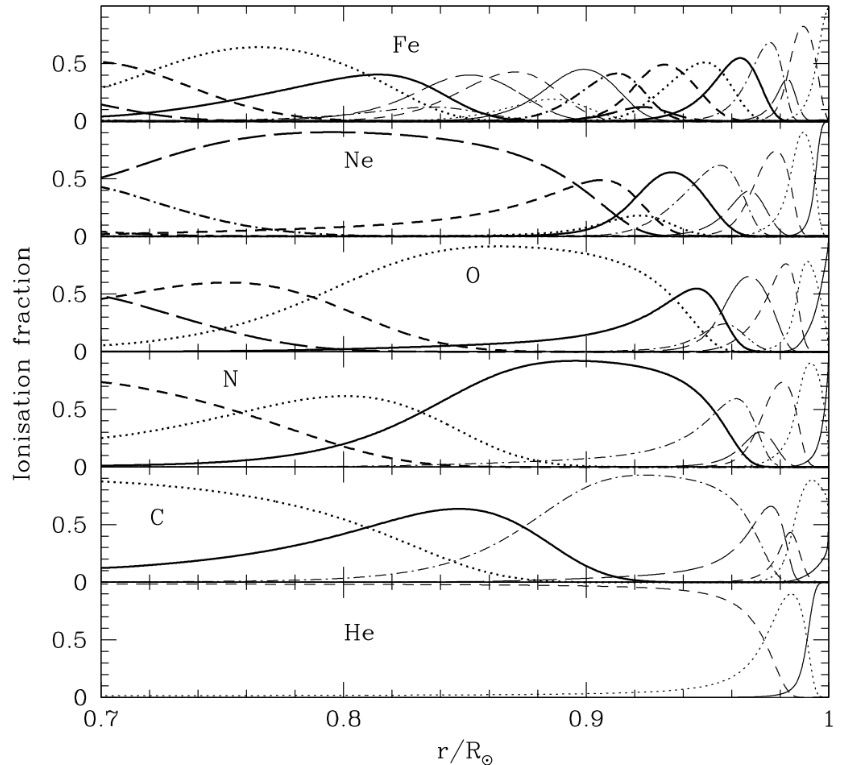
\includegraphics[width=0.4\textwidth,keepaspectratio]{ionfraction}}\label{ionfraction}
%\subcaption{Andamento di $\Gamma_1$ calcolato tramite equazione di stato MHD/OPAL. Da \cite{trampedach2006synoptic}.]{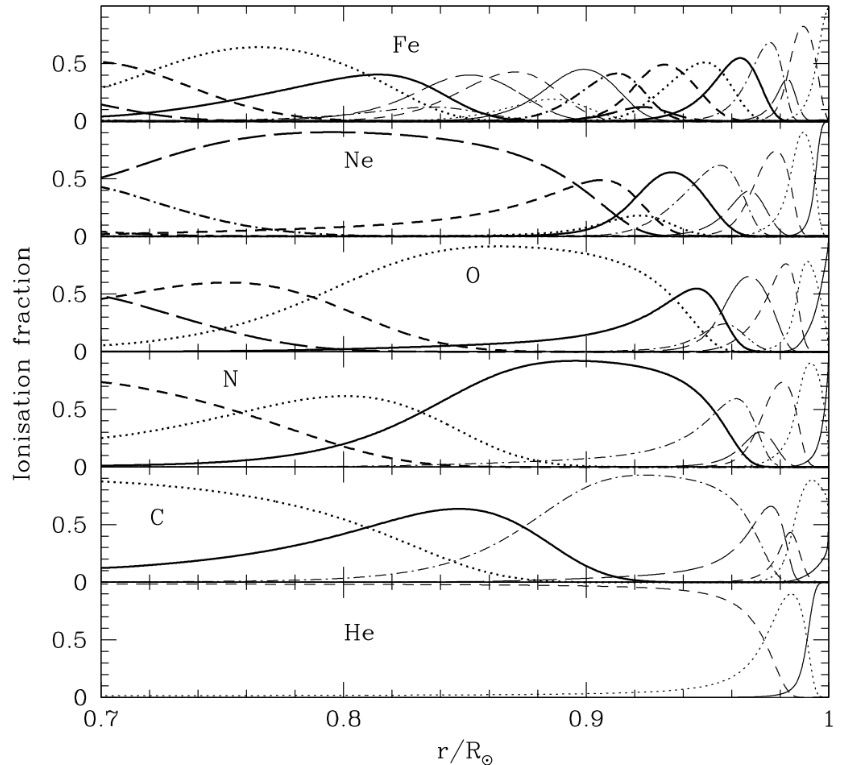
\includegraphics[width=0.4\textwidth,keepaspectratio]{ionfraction}}
~
\subfigure[Confronto $\Gamma_1$ MHD/OPAL. Da \cite{trampedach2006synoptic}.]{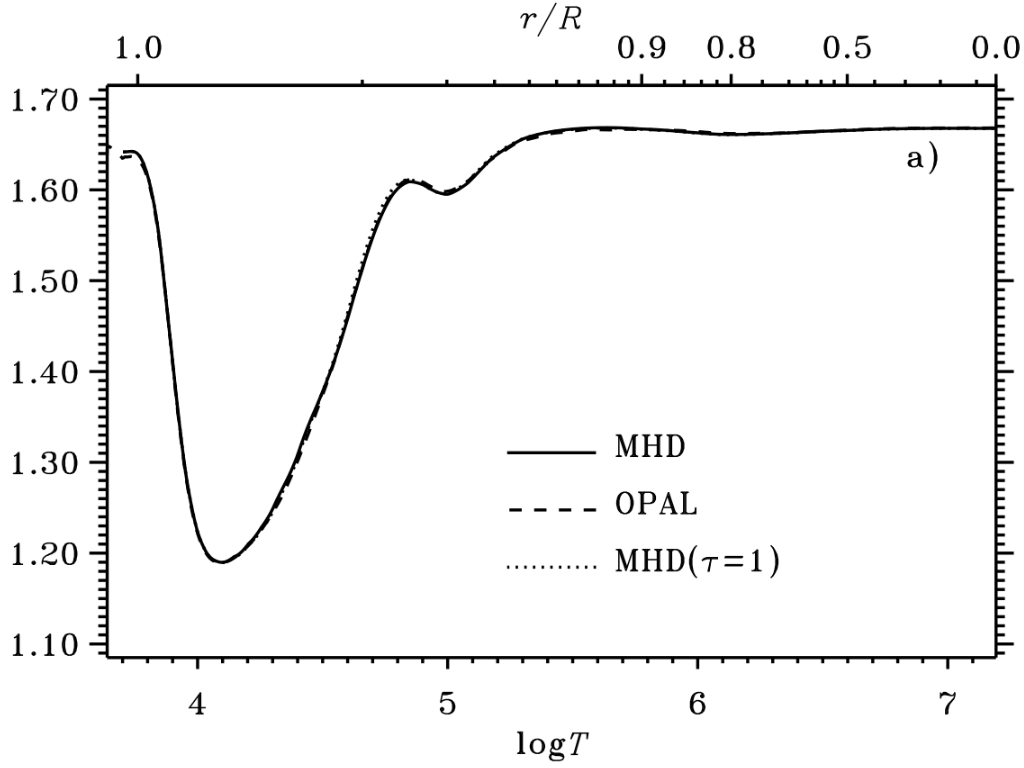
\includegraphics[width=0.4\textwidth,keepaspectratio]{gamma1eos}}
%\subcaption{Profilo radiale della popolazione dei diversi gradi di ionizzazione per $\cel{He}{4}{}{}$, CNO, $\cel{Ne}{20}{}{}$, $\cel{Fe}{56}{}{}$. Stati di ionizzazione maggiore sono pi\'u interni. Da \cite{basu2008helioseismology}.}\label{ionfraction}
%\subcaption{Andamento di $\Gamma_1$ calcolato tramite equazione di stato MHD/OPAL. Da \cite{trampedach2006synoptic}.}\label{fig:gamma1eos}
\end{figure}


\end{frame}


\subsection{Trasporto dell'energia}


\begin{frame}{T Viriale}

Il teorema del viriale esprime una propriet\'a statistica di particelle interagenti: 

L'energia potenziale gravitazionale della stella \'e
\begin{equation}
\Omega=-\int_0^M\frac{Gm(r)}{r}\,dm\label{eq:energiapg}
\end{equation}

\begin{equation}
\frac{1}{2}\TtwoDy{t}{I}=2E_i+\Omega
\end{equation}
con $E_i$ data da \eqref{eq:traslintenergy} e $I=\int r^2\,dm$. In condizioni stazionarie $\frac{1}{2}\TtwoDy{t}{I}\approx0$:
\begin{equation}
0=\int_M\frac{3P}{\rho}\,dm(r)+\Omega
\end{equation}

Detta $W=E_i+\Omega$ l'energia totale della stella, si ha:
\begin{equation}
\Omega=-2E_i\label{eq:virialegpm}
\end{equation}
e dalla conservazione dell'energia $\TDy{t}{W}+L=0$ segue che durante la fase di collasso prima dell'inizio della sequenza principale met\'a dell'energia gravitazionale viene spesa per aumentare l'energia interna e met\'a in luminosit\'a:
\begin{equation}
L=-\frac{1}{2}\dot{\Omega}=\dot{E}_i
\end{equation}

\end{frame}

\begin{frame}{Struttura in equilibrio idrostatico e termico in assenza di reazioni nucleari}

Nel caso in cui la contrazione gravitazionale sia l'unica fonte di energia per una massa gassosa in equilibrio idrostatico, il suo tempo di evoluzione caratteristico \'e il tempo di \kh{}:
\begin{equation}
\tkh{}=\frac{\Omega}{L}\approx\frac{GM^2}{2RL}\approx\SI{1.6e7}{\year}
\end{equation}

cammino libero medio degli atomi e dei fotoni sia breve, si raggiunge rapidamente l'equilibrio idrostatico e termico locale. Il processo di contrazione gravitazionale continua, su tempi-scala termodinamici, fino a che l'energia prodotta dalle reazioni nucleari bilancia l'energia irradiata.


\end{frame}


\subsection{Conservazione dell'energia interna}

\begin{frame}{Prima legge TD}

$dq$ per unit\'a di massa per $dt$:
\begin{align}
&\TDy{t}{q}=\TDy{t}{u}+P\TDof{t}(\frac{1}{\rho})\label{eq:prima}\\
%\TDy{t}{u}+P\TDy{t}{V}
&\TDy{t}{\ln{T}}=\frac{\Gamma_2-1}{\Gamma_2}\TDy{t}{\ln{P}}+\frac{\TDy{t}{q}}{c_PT}\label{eq:primatemp}\\
&\TDy{t}{\ln{P}}=\Gamma_1\TDy{t}{\ln{\rho}}+\frac{\rho(\Gamma_3-1)}{P}\TDy{t}{q}\label{eq:primapres}
\end{align}
Esponenti adiabatici $\Gamma_i$:
\begin{equation}\label{eq:adibatexp}
\Gamma_1=\Dcvar{\TDly{\rho}{P}}{Ad}, \ \Gamma_3-1=\Dcvar{\TDly{\rho}{T}}{Ad},\ \frac{\Gamma_2-1}{\Gamma_2}=\Dcvar{\TDly{P}{T}}{Ad}
\end{equation}

\end{frame}

\subsection{Equilibrio termico}

\begin{frame}{Equilibrio termico}

Scrivo il bilancio di calore per un elemento di massa unitaria di gas:
\begin{equation}
\TDy{t}{q}=\epsilon-\frac{1}{\rho}\nabla\cdot\vec{F}\label{eq:heatgl}
\end{equation}
dove $\epsilon$ \'e l'energia prodotta per unit\'a di tempo e massa e $\vec{F}$ \'e il flusso di energia verso l'esterno generalmente dovuto alla diffusione di fotoni dalla zona pi\'u calda verso la superficie; sostituendo in \eqref{eq:prima} si ha
\begin{equation}
\TDy{r}{L}=4\pi r^2[\rho\epsilon-\rho\TDof{t}u+\frac{P}{\rho}\TDy{t}{\rho}]\label{eq:fenergyconservation}
\end{equation}

Nel caso stazionario:
\begin{equation}
\TDy{t}{q}=0\ \Rightarrow\ dL=4\pi r^2\rho\epsilon\,dr
\end{equation}
e i processi nucleari che avvengono nella parte centrale forniscono il calore per bilanciare il flusso di energia irradiata.

\end{frame}

\subsection{Diffusione}

\begin{frame}{Diffusione elementi}

Velocit\'a di diffusione relativa (\citetitle{aller1960diffusion}):
\begin{equation}
v_{12}=\frac{1}{n_1}\int\,d^3v_1f_1\vec{v}_1-\frac{1}{n_{2}}\int\,d^3v_{2}f_{2}\vec{v}_{2}
\end{equation}

\begin{itemize}\label{itm:diffusionaller}
\item disomogeneit\'a di composizione
\begin{equation}
\propto\frac{1}{c_1c_{2}}\PDy{r}{c_1}
\end{equation}
\item Disomogeneit\'a pressione e forza per unit\'a di massa $F_i$:
\begin{equation}
\frac{m_{2}-m_1}{c_1m_1+c_{2}m_{2}}\frac{1}{P}\PDy{r}{P}-\frac{m_1m_{2}(\vec{F}_1-\vec{F}_{2})}{KT(c_1m_1+c_{2}m_{2})}
\end{equation}
\item disomogeneit\'a temperatura:
\begin{equation}
\frac{K_T}{n_1n_{2}}\frac{1}{T}\PDy{r}{T}
\end{equation}

\end{itemize}

$(-D_{12})/D_{12}=\frac{1}{3}lv_{th}$ con $l\approx(n\sigma)\expy{-1}$ cammino libero medio


\end{frame}

\begin{frame}{Urti}


\begin{equation}
\TDy{t}{f_i}=\PDy{t}{f_i}+\vec{v}_i\cdot\PDy{\vec{r}}{f_i}+\vec{F}_i\cdot\PDy{\vec{v}}{f_i}=-\Div_{\vec{p}}(\vec{s})=C(f_j)\label{eq:Btransport}
\end{equation}
$\tau_{diff}\approx\SI{6e13}{\year}$: soluzione dell'equazione del trasporto di Boltzmann approssimabile con la distribuzione di equilibrio traslata della velocit\'a di diffusione .

Sezione d'urto collisionale di Rutherford:
\begin{align*}
&d\sigma=\frac{4\pi(Z_iZ_j)^2}{\mu^2(\vec{v}-\vec{v}')^4}\frac{d\chi}{\chi^3}\Label{eq:dsruther}L=\int\frac{d\chi}{\chi}=\log{(\frac{1}{\chi_{min}})}\Label{eq:cL}\\
&\lambda=\max{(r_D,a_0)}:\Label{eq:maxb}
\end{align*}

\begin{align*}
\sigma_{ij}\propto \frac{e^4Z_i^2Z_j^2}{(KT)^2}\ln{\Lambda_{st}}\Label{eq:sruther}\ln{\Lambda_{ij}}\propto\ln{[1+0.18769(\frac{4KT\lambda}{Z_iZ_je^2})]}\Label{eq:clog}
\end{align*}

\end{frame}

\begin{frame}{Trasferimento impilso nelle colliioni}

Termine collisionale $C(f)$ (urti con la specie j con distribuzione $f_j$):
\begin{equation}
C(f_i,f_j)=\int\,d^3p_j\,d\sigma|\vec{v}_i-\vec{v}_j|(f_i'f_j'-f_if_j)
\end{equation}

La forza netta dovuta agli urti \'e:
\begin{align}
&\vec{R}_{ij}=\int m\vec{v}C(f_i,f_j)\,d^3v_i%\label{eq:friction}
\vec{R}_{ij}=n_in_j\mu_{ij}\alpha_{ij}\vec{V}_{ij}\label{eq:resistance}\\
&\alpha_{ij}=\frac{\mu_{ij}}{KT}\int v_r^3\sigma^Tf^{(0)}(\vec{v_r})\,d^3v_r%\label{eq:collisionintegral}
\sigma^T=\int(1-\cos{\chi})\,d\sigma\label{eq:sigmatransport}
\end{align}

\begin{block}{Diffusione termica}

La diffusione termica concentra le particelle pi\'u pesanti (e pi\'u cariche) nelle zone pi\'u calde: in presenza di un gradiente termico si ha un trasferimento netto di momento negli urti in direzione del gradiente, in \eqref{eq:friction}, dovuto al maggior numero di particelle energetiche provenienti dalle regioni pi\'u calde, ci\'o \'e dovuto alla dipendenz della sezione d'urto coulombiana dalla velocit\'a relativa $\propto v\expy{-4}$ (probabilit\'a di collisione $\propto v\expy{-3}$).

\end{block}

\end{frame}

\begin{comment}

Considero il problema in cui le due specie hanno velocit\'a relativa media diversa da zero ma piccola rispetto alla velocit\'a termica: nel sistema in cui la prima specie ha velocit\'a media nulla la seconda ha velocit\'a $V_{ij}$ quindi la distribuzione di velocit\'a della prima \'e la distribuzione di equilibrio a temperatura T quella della seconda \'e  la distribuzione di equilibrio a temperatura T traslata di $V_{ij}$, velocit\'a di diffusione:
\begin{equation}
f_j=f_j^{(0)}+\frac{m_j}{KT}(\vec{V}_{ij}\cdot\vec{v}_j)f_j^{(0)}
\end{equation}
da cui si ottiene:
\begin{align}
&\vec{R}_{ij}=n_in_j\mu_{ij}\alpha_{ij}\vec{V}_{ij}\label{eq:resistance}\\
&\alpha_{ij}=\frac{\mu_{ij}}{KT}\int v_r^3\sigma^Tf^{(0)}(\vec{v_r})\,d^3v_r\label{eq:collisionintegral}\\ &\sigma^T=\int(1-\cos{\chi})\,d\sigma\label{eq:sigmatransport}
\end{align}

\end{comment}

\begin{frame}{Sedimentazione gravitazionale}

Nella sedimentazione gravitazionale la forza per unit\'a di volume agente sulle particelle di specie i \'e
\begin{equation}
\vec{F}_i=-\nabla P_i+n_i(q_i\vec{E}+m_i\vec{g})
\end{equation}
e in condizioni di equilibrio il momento trasferito tramite urti con le altre specie \'e uguale alla forza per unit\'a di volume:
\begin{equation}
\vec{F}_i=\sum_{i\neq j}\vec{R}_{ij}%\vec{F}_{ij}=m_{ij}n_in_j\alpha_{ij}\vec{v}_{ij}
\end{equation}


In un plasma costituito da idrogeno, elio ed elettroni per mantenere la neutralit\'a la velocit\'a di diffusione degli elettroni \'e dello stesso ordine di grandezza di quella degli ioni, quindi l'impulso trasferito \'e trascurabile, da cui:
\begin{align}
&F_H\approx F_{HHe}=-\PDy{r}{P_H}+n_H(eE+m_Hg)\\
&F_{He}\approx -F_{HHe}=-\PDy{r}{P_{He}}+n_{He}(2eE+4m_Hg)\\
&E=-\frac{1}{en_e}\PDy{r}{P_e}\\
&v_{HHe}=-\frac{m_{He}T}{m_{HHe}Y\rho \alpha_{HHe}}[\PDy{r}{\ln{(P_eP_H)}}-m_Hg],\ 
n_Hv_H=\frac{(m_{He}n_Hn_{He})}{\rho}v_{HHe}\\
\end{align}

La velocit\'a di diffusione degli elementi pesanti \'e determinata prevalentemente dagli urti con H e He.
Indico con $\eta(A,r)$ la forza per unit\'a di volume sull'elemento di numero atomico Z e di massa A:
\begin{equation}\label{eq:forceperVheavy}
\begin{split}
&\eta(A,r)=-\PDy{r}{P_A}+n_A(Z_Ae\vec{E}+Am_H\vec{g})\\
&=-n_Ak_BT(\PDy{r}{\ln{P_A}}+Z_A\PDy{r}{\ln{P_e}}+\frac{AGm_HM}{r^2k_BT})
\end{split}
\end{equation}

In condizioni stazionarie si ha:
\begin{equation}\label{eq:diffheavystatinary}
\vec{F}_A\approx\vec{R}_{A,H}+\vec{R}_{A,He}=\eta(A,r)
\end{equation}
e poich\'e
\begin{equation}
\frac{\eta(A,r)}{n_Av_H(m_{A,H}n_H\alpha_{A,H})}\propto\frac{1}{XZ_A}
\end{equation}
posso trascurare $\eta(A,r)$ in \eqref{eq:diffheavystatinary} ed esplicitando i contributi $R_{A,H}$ e $R_{A,He}$
ottengo
\begin{equation}\label{eq:diffvelocityA}
v_A(1+2\frac{Y}{X})\approx-v_H
\end{equation}
%&n_Av_A(m_{AH}n_Hw_{AH})(1+2\frac{Y}{X})\approx-n_Av_H(m_{AH}n_Hw_{AH})

\end{frame}

\begin{comment}%%Contributi alla velocit\'a di diffusione di H-He in modello solare. Da \cite{wam88hydrogen}%
\begin{minipage}{\linewidth}
\begin{tikzpicture}
\node[inner sep=0pt] (image) at (0,0)
  {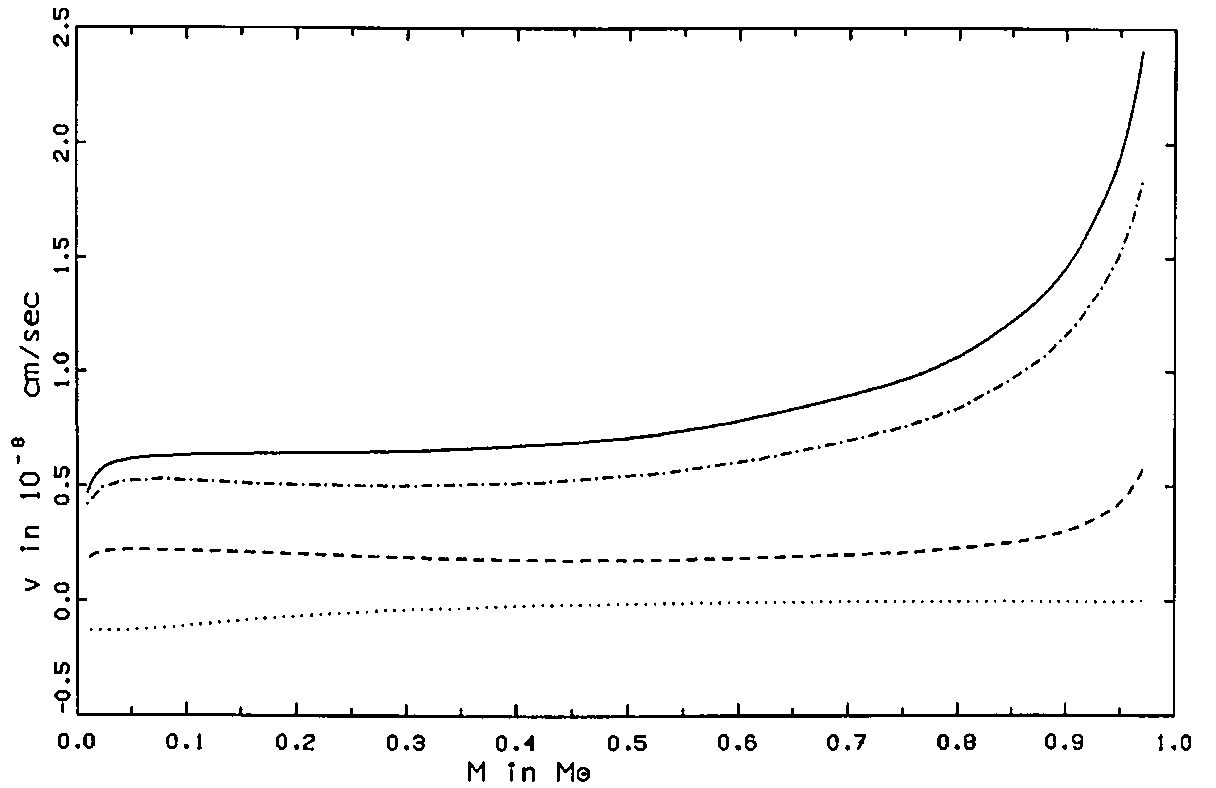
\includegraphics[keepaspectratio=true,width=0.5\textwidth]{Hdiffusion}};
  \draw [thick,dotted] (-3.4,1.5) -- (-3,1.5) node[right] {$\propto\nabla c$};
 \draw [thick,dashed] (-3.4,1.9) -- (-3,1.9) node[right] {$\propto\nabla T$};
    \draw [thick,dash dot] (-3.4,2.3) -- (-3,2.3) node[right] {$\propto\nabla P$};
    \node (caption) at (8.5,-2.5) { \begin{minipage}[c]{0.48\textwidth}
\captionof{figure}{Contributi alla velocit\'a di diffusione di H-He in modello solare. Da \cite{wam88hydrogen}.}%   
    \end{minipage}};
\node[] (massconsdiff) at (8.5,1) {\begin{minipage}[c]{0.48\textwidth}
\end{minipage}
};
\end{tikzpicture}
\end{minipage}
\end{comment}


\section{Trasporto di energia}

\subsection{Trasporto radiativo.}

\begin{frame}{Trasporto radiativo}

$\frac{1}{\kappa\rho}\approx\SI{1}{\cm}$, con $\kappa$ opacit\'a radiativa per unit\'a di massa, quindi considero la radiazione localmente in equilibrio con la materia
%Il flusso di energia verso la superficie \'e generato da una piccola anisotropia nell'intensit\'a descritta al prim'ordine tramite:
\begin{align}
I_{\nu}=B(\nu,T)-\frac{1}{\kappa_{\nu}'\rho}\nabla_s B(\nu,T)\\
P_{rad}=\int\,d\nu\frac{4\pi}{3c}B_{\nu}=\frac{1}{3}aT^4\\
\vec{F}=-\frac{4\pi}{3\kappa\rho}\nabla B=-\frac{4\pi}{3\kappa\rho}\nabla B=-\frac{c}{\kappa\rho}\nabla P_{rad}\\
\nrad{}=\Dcvar{\PDly{P}{T}}{rad}=\frac{3}{16\pi acG}\frac{\kappa l(r)P}{m(r)T^4}\label{eq:radiativegradient}
\end{align}

\end{frame}

\subsection{Opacit\'a.}

\begin{frame}{Opacit\'a media di Rosseland}

\begin{equation}
\frac{1}{\kappa}=(\frac{acT^3}{\pi})\expy{-1}\intzi{}\,d\nu\frac{1}{\kappa_{\nu}}\PDy{T}{B(\nu,T)}\label{eq:rosselandopacity}
\end{equation}

\begin{itemize}[noitemsep,topsep=0pt,parsep=0pt,partopsep=0pt]

\item Scattering fotone-elettrone (sc). Scattering Thomson per $h\nu\ll m_ec^2$ (Scattering Compton per $T\geq\SI{e8}{\kelvin}$)
\begin{align}
&\kappa_{\nu}\propto\frac{r_e^2}{\mu_em_u}, \kappa_{sc}=0.20(1+X)\si{\squared\cm\per\gram}
%&r_e=\SI{2.82e-13}{\cm}
\end{align}


\item Brehmstrahlung inverso (ff).
\begin{equation}
\kappa_{ff}\propto\rho T\expy{-\frac{7}{2}}
\end{equation}
Effetti quantistic: fattore di Gaunt.

\item Reazioni di ionizzazione (bf).
\begin{equation}
\sigma_{bf}=\num{2.82e29}\frac{Z^4}{n^5\nu^3}g(\nu,n,l,Z)\si{\square\cm}
\end{equation}

\item Transizione elettronica a livelli eccitati (bb).

\item Scattering atomici e ione $H^-$. $H^-$:$h\nu>\SI{0.75}{\ev}/\lambda<\SI{1655}{\nano\meter}$.

\end{itemize}

\end{frame}

\begin{frame}{Profilo radiale $\kappa$}

\begin{figure}[!ht]
\centering
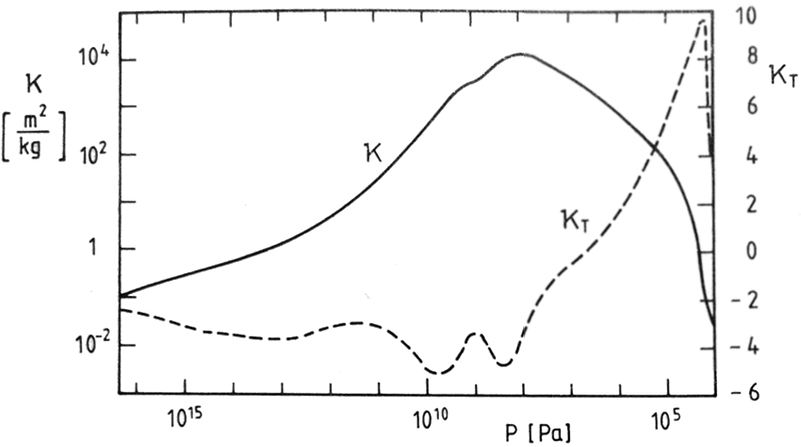
\includegraphics[keepaspectratio,width=0.9\linewidth]{opacitylld}
\caption{Profilo radiale di $\kappa$ e $\PDly{T}{\kappa}$. Da \cite{stix91sun}.}
\end{figure}

\end{frame}

\begin{frame}{Contributi a $\kappa$ per processoper elemento}

\begin{tikzpicture}[]
%([shift={(1.5,0)}]0,0)

\node[anchor=north west] (opint) at (0,0) {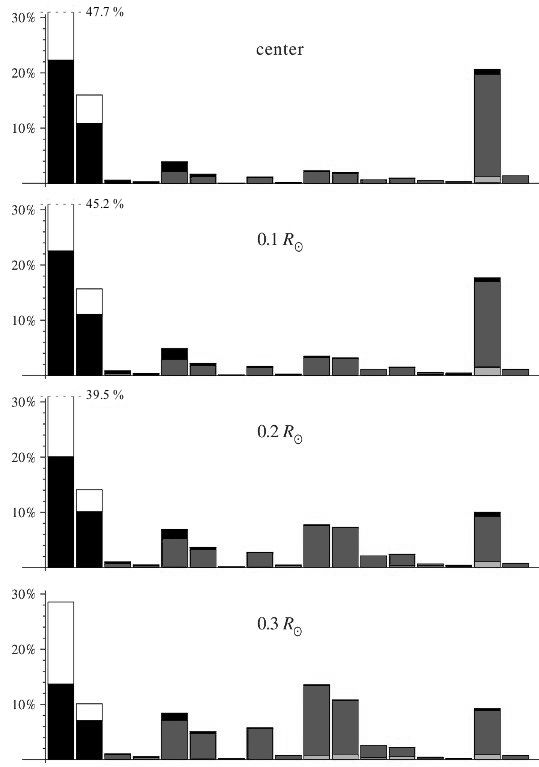
\includegraphics[width=0.45\textwidth,keepaspectratio]{opcontrib-int-g}};
\node[anchor=west,right=2.5cm of opint.east] (opout) {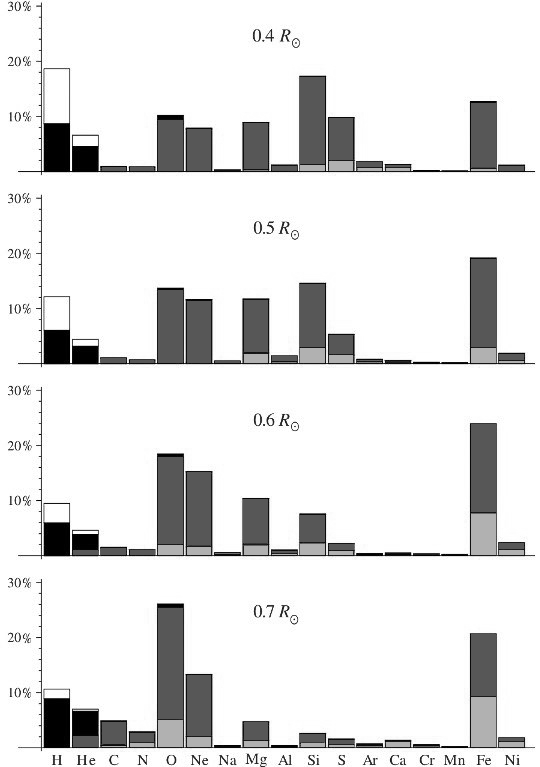
\includegraphics[width=0.45\textwidth,keepaspectratio]{opcontrib-out-g}};
\begin{scope}[scale=0.6]
\node[draw,anchor=west,label={[label distance=2mm]-90:Scattering \Pphoton\Pelectron},minimum size=5mm,below right=1cm and 9mm of opint.east] (sc) {};
\node[draw,label={[label distance=2mm]-90:ff},fill=black,minimum size=5mm,above=10mm of sc] (ff) {};
\node[draw,label={[label distance=2mm]-90:bb},fill=bb,minimum size=5mm,above=10mm of ff] (bb) {};
\node[draw,label={[label distance=2mm]-90:bf},fill=bf,minimum size=5mm,above=10mm of bb] (bf) {};
\end{scope}

\begin{scope}[node distance=2.62mm]
\node[minimum size=2mm,name=hydrogen, right=6.5mm of opint.south west] {\tiny H};
\node[minimum size=2mm,name=helium, right=of hydrogen.west] {\tiny He};
\node[minimum size=2mm,name=carbonium, right=of helium.west] {\tiny C};
\node[minimum size=2mm,name=nitrum, right=of carbonium.west] {\tiny N};
\node[minimum size=2mm,name=oxygen, right=of nitrum.west] {\tiny O};
\node[minimum size=2mm,name=neon, right=of oxygen.west] {\tiny Ne};
\node[minimum size=2mm,name=sodium, right=of neon.west] {\tiny Na};
\node[minimum size=2mm,name=magnesium, right=of sodium.west] {\tiny Mg};
\node[minimum size=2mm,name=alluminium, right=of magnesium.west] {\tiny Al};
\node[minimum size=2mm,name=silicium, right=of alluminium.west] {\tiny Si};
\node[minimum size=2mm,name=sulfur, right=of silicium.west] {\tiny S};
\node[minimum size=2mm,name=argon, right=of sulfur.west] {\tiny Ar};
\node[minimum size=2mm,name=calcium, right=of argon.west] {\tiny Ca};
\node[minimum size=2mm,name=cromum, right=of calcium.west] {\tiny Cr};
\node[minimum size=2mm,name=manganese, right=of cromum.west] {\tiny Mn};
\node[minimum size=2mm,name=ferrum, right=of manganese.west] {\tiny Fe};
\node[minimum size=2mm,name=nikel, right=of ferrum.west] {\tiny Ni};

\end{scope}
 
\node[anchor=north west, below right=1mm and 0.5cm of opint.south west] {\parbox{\textwidth}{\captionof{figure}{Importanza dei varii contributi all'opacit\'a nell'interno solare; composizione GS98. Da \cite{bla11opacity}.}\label{fig:opacitycontrib} }};
 
\end{tikzpicture}

\end{frame}


\subsection{Condizione di in-stabilit\'a dinamica: trasporto convettivo.}

\begin{frame}{Stabilit\'a convettiva}

\begin{equation}
\rho\PtwoDy{t}{(\Delta r)}=-g\Delta\rho=-g[\Dcvar{\TDy{r}{\rho}}{e}-\Dcvar{\TDy{r}{\rho}}{amb}]\Delta r
\end{equation}

\begin{align}
&\frac{d\rho}{\rho}=\alpha\frac{dP}{P}-\delta\frac{dT}{T}+\phi\frac{d\mu}{\mu}\label{eq:deltatherm}
\end{align}

\begin{equation}
\PtwoDy{t}{(\Delta r)}=-g\frac{\delta}{H_P}[\nabla_e-\nabla-\frac{\phi}{\delta}\nmu{}]\Delta r=-N^2\Delta r
\label{eq:galleggiamento}
\end{equation}
\begin{equation}
\nabla_e\approx\nabla_{ad}=\frac{P\delta}{T\rho c_P}
\end{equation}
Vedi STELLAR STRUCTURE  AND EVOLUTION - Mechanical and thermal equilibrium - Equation of state of stellar interiorsPg 32
\begin{equation}
N^2=g(\frac{1}{\Gamma_1P}\TDy{r}{P}-\frac{1}{\rho}\TDy{r}{\rho})=g(\frac{1}{\densityscale{}}-\frac{g}{c_s^2})\label{eq:bvfs}
\end{equation}



\begin{equation}
\nrad{}<\nad+\frac{\phi}{\delta}\nmu{}\label{eq:ledoux}
\end{equation}

\end{frame}

Le stelle con massa $M\leq1.1\msun{}$ hanno una regione radiativa interna mentre la parte esterna \'e convettiva: la regione in cui vale l'uguaglianza in \eqref{eq:ledoux} \'e la base della zona convettiva, la cui posizione \'e determinata dall'aumentare dell'opacit\'a col diminuire della temperatura.
% e dal gradiente adiabatico, il cui valore \'e diminuito dal calore latente di idrogeno ed elio nelle regioni di ionizzazione parziale.

Una maggiore efficienza del trasporto convettivo di energia si riflette in una minore differenza tra il gradiente di temperature adiabatico ed effettivo.

\begin{figure}[!h]
    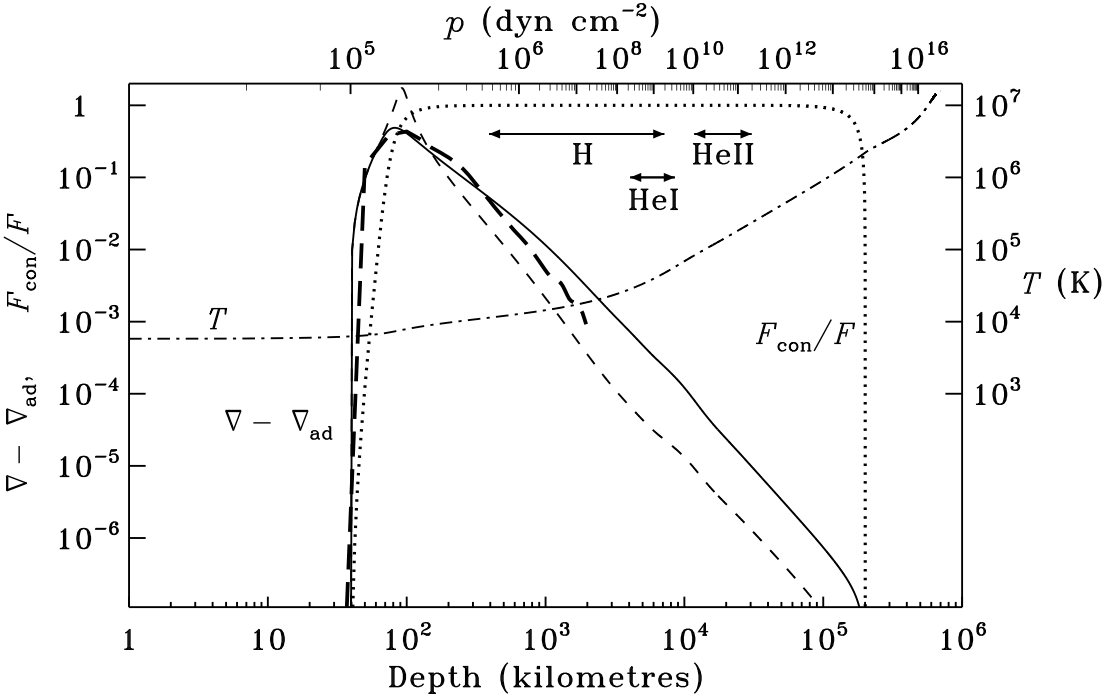
\includegraphics[width=0.9\textwidth,keepaspectratio]{proportionflux}
    \caption{Profilo radiale (profondit\'a in \si{\kilo\meter}) del flusso convettivo $F_c$ rispetto al flusso totale $F$, della super-adiabaticit\'a $\nabla-\nad{}$ e regioni di ionizzazione idrogeno e $\cel{He}{4}{}{}$. Da \cite{gou76convection}.}
    \label{fluxproportion}
\end{figure}

\subsection{Teoria della mixing-length.}

In presenza di convezione il flusso di energia verso l'esterno ha una componente radiativa, determinata dal gradiente di temperatura, e una componente dominante convettiva 
\begin{equation}
F=F_{con}+F_{rad}=\frac{\lsun{}}{4\pi r^2}
\end{equation}
Definisco il gradiente radiativo fittizio:
\begin{equation}
F=\frac{4acG}{3}\frac{T^4m}{\kappa Pr^2}\nrad{}\label{eq:fictionrad}
\end{equation}

Per determinare il gradiente di temperatura effettivo $\nabla$ uso la teoria della mixing-length (\cite{prandtl25tur} e \cite{vitense53kon}):
si considera l'eccesso di calore trasportato dai blob di gas nel moto convettivo $c_P\Delta T$ rispetto all'ambiente, il cui cammino libero medio \'e la mixing-length $l_m=\alpha H_P$, che da luogo al flusso di energia

\begin{equation}
F_{con}=\exv{\rho vc_P\Delta T}\label{eq:convectiveflux}
\end{equation}

dove $\exv{}$ indica una media opportuna sulla sfera di raggio r. Determino il valor medio della differenza di temperatura prendendo come valore caratteristico dello spostamento del blob, considerando moti in entrambi i versi, $\Delta r\approx\frac{l_m}{2}$:
\begin{equation}
\frac{\Delta T}{T}\approx\frac{1}{T}\PDy{r}{(\Delta T)}\frac{l_m}{2}=(\nabla-\nabla_e)\frac{l_m}{2}\frac{1}{H_P}
\end{equation}

Assumo il lavoro medio fatto dalla forza di galleggiamento per unit\'a di massa $-g\frac{\Delta\rho}{\rho}$ uguale al valore medio della forza, cio\'e la met\'a di quello alla superficie sferica data, moltiplicato lo spostamento medio $\frac{l_m}{2}$ quindi, assumendo in oltre che in media met\'a del lavoro fatto dalla forza di galleggiamento sia trasformato in energia cinetica del blob si ottiene

\begin{equation}
v^2=g\delta(\nabla-\nabla_e)\frac{l_m^2}{8H_P}\label{eq:blobvelocity}
\end{equation}

Infine determino gli scambi radiative del blob: il modulo del flusso radiativo \'e proporzionale al gradiente termico in direzione normale alla superficie del blob
\begin{equation}
f=\frac{4acT^3}{3\kappa\rho}|\PDy{n}{T}|
\end{equation}
quindi l'energia scambiata dall'intera superficie S del blob \'e $\lambda=Sf$ che determina, per la prima legge della termodinamica, una variazione di temperatura per unit\'a di tempo:
\begin{equation}
\PDy{t}{T_e}=-\frac{\lambda}{\rho Vc_P}
\end{equation}
indicato con $V$ il volume del blob.

La variazione della temperatura del blob per unit\'a distanza percorsa \'e quindi
\begin{equation}
\Dcvar{\TDy{r}{T}}{e}=\Dcvar{\TDy{r}{T}}{ad}-\frac{\lambda}{\rho Vc_Pv}\label{eq:Tchangelength}
\end{equation}
e approssimando il gradiente normale alla superficie con $\exv{\Delta T}$ ed usando le definizioni \eqref{eq:nablavitense} si ottiene:
\begin{equation}
\frac{\nabla_e-\nad{}}{\nabla-\nabla_e}=\frac{6acT^3}{\kappa\rho^2c_Pl_mv}
\end{equation}

Le 5 equazioni \eqref{eq:fictionrad},\eqref{eq:radiativegradient}, \eqref{eq:convectiveflux}, \eqref{eq:blobvelocity}, \eqref{eq:nablavitense} determinano completamente le variabili $F_{rad}, F_{con}, v, \nabla_e, \nabla$ in funzione di $P,T,l(r),m(r),c_P,\nad{},\nrad{},g$ .



\section{Produzione di energia - reazioni di fusione}

\begin{frame}{Sezione d'urto di fusione}
L'energia liberata dalle reazioni nucleari per grammo per secondo $\epsilon(\rho,T,X_i)$ \'e determinata dalla probabilit\'a che la reazione $X(a,b)Y$ abbia luogo. Sia $E$ l'energia cinetica nel centro di massa dei nuclei, la sezione d'urto $\sigma(E)$ di fusione \'e:
\begin{equation}
\sigma(E)=\pi\lambdabar^2P_0(E)S(E)
\end{equation}

La lunghezza d'onda di de Broglie relativa delle particelle descrive l'indeterminazione sulla posizione nell'urto di due particelle con momento relativo p:
\begin{equation}
\lambdabar=\frac{\hbar}{p}=\frac{\hbar}{\sqrt{2mE}}
\end{equation}

Il fattore astrofisico $S(E)$ descrive l'interazione tra i due reagenti a livello nucleare ed \'e debolmente dipendente dall'energia lontano da risonanze.

La probabilit\'a di attraversamento della barriera coulombiana \'e:
\begin{equation}
P_0(E)=\exp{-2\pi\eta},\ \eta=\sqrt{\frac{m}{2}}\frac{Z_1Z_2e^2}{\hbar E\expy{\frac{1}{2}}}
\end{equation}
Scrivo la sezione d'urto per i nuclei di carica $Z_1$, $Z_2$ e m massa ridotta:
\begin{equation}
\sigma(E)=\frac{S(E)}{E}\exp{-2\pi\eta}\label{eq:fusioncrosssection}
\end{equation}

La funzione $\epsilon(\rho,T,X_i)$ \'e determinata dalla somma di tutti i contributi
\begin{equation}
\epsilon_{ij}=\frac{1}{1+\delta_{ij}}Q_{ij}\frac{\rho N_A^2X_jX_k}{{A_jA_k}}\exv{\sigma v}\label{eq:energyrate}
\end{equation}
dove $Q_{ij}$ \'e l'energia liberata per reazione tra nucleo di specie i e j; $X_i$ indica la frazione in  massa della specie i; $\exv{}$ indica la media sulla distribuzione di Maxwell-Boltzmann
\begin{equation}
f(E)dE\propto\frac{E\expy{\frac{1}{2}}}{(kT)\expy{\frac{3}{2}}}\exp{-\frac{E}{kT}}\,dE\label{eq:MB}
\end{equation}

Per determinare $\exv{\sigma v}$ uso il fatto che l'integrando
\begin{equation}
S(E)\exp{-\frac{E}{kT}-\frac{b}{\sqrt{E}}}\label{eq:reactionrateM}
\end{equation}
ha forma approssimativamente gaussiana il cui massimo $E_G$, energia pi\'u probabile di reazione, e FWHM sono:
\begin{equation}
E_G=\SI{5.665}{\kilo\ev} A\expy{\frac{1}{3}}T_7\expy{\frac{2}{3}},\ \Delta E=4.249W\expy{\frac{1}{6}}T_7\expy{\frac{5}{6}}
\end{equation}
posto $W=Z_j^2Z_k^2A=Z_j^2Z_k^2\frac{A_iA_j}{A_i+A_j}$.

Il rate locale per reazioni non risonanti si scrive approssimativamente come:
\begin{equation}
\exv{\sigma v}=\num{1.3005e-15}[\frac{Z_1Z_2}{AT_6^2}]\expy{\frac{1}{3}}fS_{eff}\exp{-\tau}\si{\cubic\cm\per\second},\ \tau=\frac{3E_G}{kT}\approx\num{42.487}(Z_1^2Z_2^2AT_6\expy{-1})\expy{\frac{1}{3}}
\end{equation}
$S_{eff}$ \'e il risultato dell'espansione dell'integrando per $\invers{\tau}\ll1$ ed estrapolato a $E_G$ a partire dal valore a $E(0)$ determinato dalla fisica nucleare.

\end{frame}

\begin{frame}{Reazioni catena PP}


\setmuskip{\thinmuskip}{0mu}\setmuskip{\medmuskip}{0mu}
\tikzset{->-/.style={decoration={
  markings,
  mark=at position .5 with {\arrow{>}}},postaction={decorate}},
-->/.style={decoration={
  markings,
  mark=at position .8 with {\arrow{>}}},postaction={decorate}},
box/.style={%
%draw,
minimum width=25mm,%
    minimum height=6mm,%
    align=center}
}

\begin{tikzpicture}

\begin{scope}[scale=0.8,transform shape]
\node[box] (pp) at (0,0) {$\Pproton{+}\Pproton{\to}\cel{H}{2}{}{}{+}\Pnue{+}\APelectron$};%%pp
\node[box,right=2cm of pp]  (pep) {$\Pproton{+}\Pproton{+}\Pelectron{\to}\cel{H}{2}{}{}+\Pnue$};%%pep
\coordinate[below=0.3cm of pp] (bpp);
\node[left] at (bpp) {$99.76\%$};
\coordinate[below=0.3cm of pep] (bpep);
\node[right] at (bpep) {$0.24\%$};

\coordinate[] (ttriton) at ($(bpp)!0.5!(bpep)$);
\draw[->-] (pp)--(bpp)--(ttriton);
\draw[->-] (pep)--(bpep)--(ttriton);
\node[box,below=0.3cm of ttriton] (triton) {$\Pproton+\cel{H}{2}{}{}\to\cel{He}{3}{}{}+\Pphoton$};%%triton
\coordinate[below=0.3cm of triton] (btriton);
\draw[-->] (ttriton)--(triton.north);
\draw[->-] (triton.south)--(btriton.north);
\coordinate[left=2.5cm of btriton] (tpp1);
\node[left] at (tpp1) {$83.3\%$};
\coordinate[right=2.0cm of btriton] (tberillium7);
\node[above] at (tberillium7) {$16.7\%$};
\coordinate[right=6.5cm of btriton] (thep);
\node[right] at (thep) {$\num{2e-5}\%$};

\draw[] (btriton)--(tpp1);
\draw[] (btriton)--(tberillium7);
\draw[] (tberillium7)--(thep);
\node[box,below=0.5cm of tpp1,label={[xshift=0.1cm, yshift=-1.5cm]PPI}]  (pp1) {$\cel{He}{3}{}{}+\cel{He}{3}{}{}\to\cel{He}{4}{}{}+2\Pproton$};%%pp1
\node[box,below=0.5cm of tberillium7]  (berillium7) {$\cel{He}{3}{}{}+\cel{He}{4}{}{}\to\cel{Be}{7}{}{}+\Pphoton$};%%berillium7
\node[box,below=0.5cm of thep,label={[xshift=-0.1cm, yshift=-1.5cm]HEP}]  (hep) {$\cel{He}{3}{}{}+\Pproton\to\cel{He}{4}{}{}+\APelectron+\Pnue$};%%hep

\draw[->-] (tpp1)--(pp1.north);
\draw[->-] (tberillium7)--(berillium7.north);
\draw[-->] (thep)--(hep.north);

\coordinate[below=0.3cm of berillium7] (bberillium7);
\coordinate[left=1.5cm of bberillium7] (tlithium7);
\node[left] at (tlithium7) {$99.88\%$};
\coordinate[right=2.0cm of bberillium7] (tboron8);
\node[right] at (tboron8) {$0.12\%$};

\node[box,below=0.5cm of tlithium7]  (li7) {$\cel{Be}{7}{}{}+\Pelectron\to\cel{Li}{7}{}{}+\Pnue$};%%Li7
\node[box,below=0.5cm of li7,label={[xshift=0.1cm, yshift=-1.5cm]PPII}] (pp2) {$\cel{Li}{7}{}{}+\Pproton\to2\cel{He}{4}{}{}$};%% PP2

\node[box,below=0.5cm of tboron8]  (b8) {$\cel{Be}{7}{}{}+\Pproton\to\cel{B}{8}{}{}+\Pphoton$};%%B8
\node[box,below=0.25cm of b8]  (be7) {$\cel{B}{8}{}{}\to\cel{Be}{8}{}{}^*+\APelectron+\Pnue$};%%Be8*
\node[box,below=0.25cm of be7,label={[xshift=0.1cm, yshift=-1.5cm]PPIII}]  (pp3) {$\cel{Be}{8}{}{}^*\to2\cel{He}{4}{}{}$};%%pp3

\draw[->-] (berillium7.south)--(bberillium7);
\draw[] (bberillium7)--(tlithium7);
\draw[] (bberillium7)--(tboron8);

\draw[->-] (tlithium7)--(li7.north);
\draw[->-] (li7.south)--(pp2.north);

\draw[->-] (tboron8.south)--(b8.north);
\draw[->-] (b8.south)--(be7.north);
\draw[->-] (be7.south)--(pp3.north);
\end{scope}

\node[anchor=north west]  at ($(0,0)+(-50mm,-1mm)$) {\parbox{0.5\textwidth}{\captionof{figure}{Reazioni catena PP: terminazioni per temperature caratteristiche del centro solare. Da \cite{adelberger2011solar}.}}};

\end{tikzpicture}

\end{frame}

\begin{frame}{Fattore astrofisico}
\centering
\begin{tikzpicture}[ampersand replacement=\&]

\begin{scope}[scale=0.5,transform shape,every node/.style={scale=0.6}]
\node [matrix,ampersand replacement=\&, matrix of nodes,column sep={60pt,between origins},row
    sep={15pt,between origins}] (s)
  {
Reazione \&  $S(0) (keVb)$ \& \parbox{2cm}{\centering Incertezza su $S(E_G) (\%)$}\\
$p(p,\APelectron\Pnue)d$ \& $(4.01 \pm 0.04)10^{-22}$ \& $\pm 0.7$\\
$d(p,\Pphoton)\cel{He}{3}{}{}$ \& ${2.14}10^{-4}\substack{+0.17 \\ -0.16}$ \& $\pm 7.1$\\
$\cel{He}{3}{}{}(\cel{He}{3}{}{},2p)\cel{He}{4}{}{}$ \& $(5.21 \pm 0.27)10^{-3}$ \& $\pm 4.3$\\
$\cel{He}{3}{}{}(\cel{He}{4}{}{},\Pphoton)\cel{Be}{7}{}{}$ \& $0.56 \pm 0.03$ \& $\pm 5.1$\\
$\cel{He}{3}{}{}(p,\APelectron\Pnue)\cel{He}{4}{}{}$ \& $(8.6 \pm 2.6)10^{-20}$ \& $\pm 30$\\
$\cel{Be}{7}{}{}(\Pelectron,\Pnue)\cel{Li}{7}{}{}{\ }^{I}$ \& $ $ \& $\pm 2.0$\\
$p(p\Pelectron,\Pnue)d{\ }^{II}$\& $ $ \& $\pm 1.0$\\
$\cel{Be}{7}{}{}(p,\Pphoton)\cel{B}{8}{}{}$\& $(2.08 \pm 0.16)10^{-2}$ \& $\pm 7.5$\\
%14N(p,7)150 XI.A 1.66 \pm 0.12 (-3.3 \pm 0.2) x 10-3 b (4.4 \pm 0.3) x 10-5 a \pm 7.2
  };
\draw[]({$(s-1-1)!.5!(s-1-2)$} |- s.north) -- ({$(s-1-1)!.5!(s-1-2)$} |- s.south);
\draw[]({$(s-1-2)!.5!(s-1-3)$} |- s.north) -- ({$(s-1-2)!.5!(s-1-3)$} |- s.south);
\node[fit=(s-1-1.south) (s-1-2.south) (s-1-3.south),inner sep=0pt] (R2) {};
\draw[] (R2.south -| s.west) -- (R2.south -| s.east);
 \end{scope}
 
\node (pep) at ($(s.south)+(47mm,-6mm)$) {\parbox{\textwidth}{\begin{equation*}\scriptscriptstyle II: R(p\Pelectron p)=\scriptscriptstyle1.102(1\pm0.01)10^{-4}\midfrac{\rho}{\mu_e}T_6\expy{-1/2}
\scriptscriptstyle[1+0.002(T_6-16)]R(pp)\end{equation*}}};
\node[below=0.1mm of pep] (ec) {\parbox{\textwidth}{\begin{equation*}\scriptscriptstyle I: R(\cel{Be}{7}{}{}(\Pelectron,\Pnue)\cel{Li}{7}{}{})=\scriptscriptstyle5.6(1\pm0.02)10^{-9}\midfrac{\rho}{\mu_e}T_6\expy{-1/2}\scriptscriptstyle[1+0.004(T_6-16)]\si{\per\second}\end{equation*}}};
 
\node[below=0.1mm of ec] (captions) {\parbox{\textwidth}{\captionof{figure}{Fattore astrofisico reazioni catena PP}}};

\end{tikzpicture}

\end{frame}

\begin{frame}{Schermaggio elettronico}

\begin{figure}[!ht]
       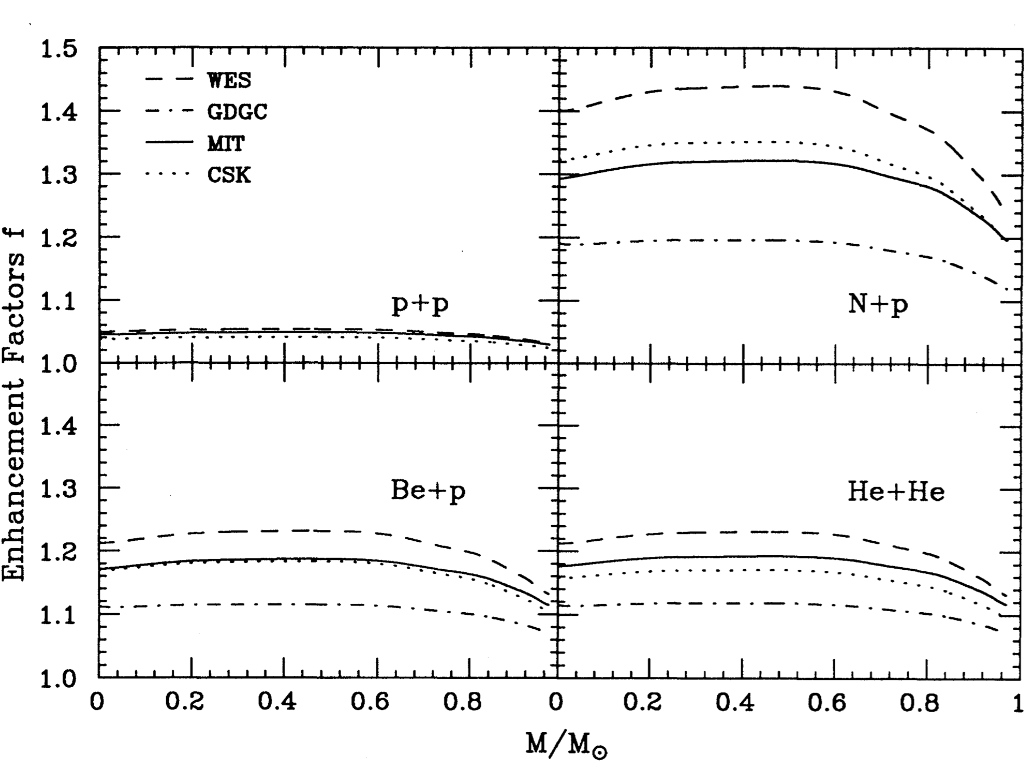
\includegraphics[width=0.4\textwidth,keepaspectratio]{Rscreening}
       \caption{Andamento della correzione di schermaggio degli elettroni secondo diversi schemi. Da \cite{ricci1995screening}.}
\end{figure}

L'energia potenziale dovuta all'interazione di due nuclei $Z_1$ e $Z_2$ a distanza r contiene un contributo delle altre cariche presenti nel plasma:
\begin{equation}
U=\frac{Z_1Z_2e^2}{r}+U_s(r_{12})
\end{equation}
dove il primo termine \'e l'energia potenziale non schermata e il termine $U_s(r_{12})$ il contributo della nuvola elettronica. L'effetto di $U_s$ \'e di aumentare la probabilit\'a di attraversamento della barriera coulombiana. Correggo quindi \eqref{eq:fusioncrosssection} con il fattore moltiplicativo:
\begin{equation}
f=\exp{-\midfrac{U_0}{KT}}\label{eq:screeningfactor}
\end{equation}
dove $U_0=U_s(0)$ poich\'e $r\ll r_D$ e considerando solo la correzione al fattore di penetrazione ($E_G\gg U_0$).

Per determinare $U_0$ considero l'energia potenziale di $Z_1$ e $Z_2$ a distanza $r$
\begin{equation}
U=Z_2e\int_{\infty}^r\PDy{r_1}{\phi_1}\,dr_1=\frac{Z_1Z_2e^2\exp{-\midfrac{r}{r_D}}}{r}
\end{equation}
con $\phi_1$ dato da \eqref{eq:screenedpotential}, e quindi
\begin{equation}
U_s=U-\frac{Z_1Z_2e^2}{r}
\end{equation}

\end{frame}

\begin{frame}{Tempo in sequenza principale}

Sulla base dell'efficienza delle reazioni nucleari, del profilo di densit\'a e temperatura ricavati da un modello solare le terminazione della catena pp $\cel{He}{3}{}{}-\cel{He}{3}{}{}$ e $\cel{He}{3}{}{}-\cel{He}{4}{}{}$ generano rispettivamente $83.3\%$, $16.7\%$ della luminosit\'a totale mentre il ciclo CNO circa $1\%$.

Il tempo trascorso da una stella di massa solare in sequenza principale considerando \'e il tempo necessario per la massa di idrogeno nel core di fusione (le temperature necessarie perch\'e il rate di reazione sia apprezzabile si raggiungono nella regione pi\'u interna che costituisce una frazione $f$ pari al $15\%$ della massa solare) ad esaurirsi:

\begin{equation}
\tau_n\approx\frac{E_n}{L}=\frac{fX\msun Q}{\lsun}\approx\SI{e+10}{\year},\ Q\approx\SI{6.3e18}{\erg\per\gram}
\end{equation}

\end{frame}

\section{Modello solare standard e osservabili sismologiche}




%%% SOS
%\part{OSCILLAZIONI SOS}
%\subsection{Osservabili stellari}

\begin{frame}<1>[label=noinside]{Modello stellare}{Come indagare la fisica interna a una stella?}

\onslide<1->\begin{block}{Osservabili stellari:}
$L$, $M$, $R$, $T_e$, $(\frac{Z}{X})_{ph}$, $g_{ph}$.
\end{block}

\onslide<1->\begin{block}{Informazioni sulla struttura interna?} Condizione di equilibrio idrostatico
\end{block}

%Teorema Vogt-Russel: $X_i(r)$, $M$ \pause equilibrio (idrostatico/termico) determinano struttura stellare .
%\pause

\onslide<1->\begin{block}{Modello stellare: diagramma di \hr{}.}
\end{block}

\onslide<2->\begin{block}{Descrizione fisica interno stellare: parametri aggiuntivi}
Convezione, diffusione e sedimentazione elementi pesanti, equazione di stato, opacit\'a
\end{block}

\onslide<2->\begin{block}{Astrosismologia}
Restringo spazio parametri sistemi stellari lontani
\end{block}

\end{frame}


{ % all template changes are local to this group.
    \setbeamertemplate{navigation symbols}{}
    \begin{frame}[plain]{Diagramma di \hr{}}
        \begin{tikzpicture}[remember picture,overlay]
            \node[at=(current page.center)] {
                %\includegraphics[width=\paperwidth]{yourimage}
            };
        \end{tikzpicture}
     \end{frame}
}



\againframe<2>{noinside}


\section{Osservazioni}

\subsection{Fitting polinomiale: inversione ''1.5-D''.}

\begin{frame}<1>[label=noinside]{Modello stellare}{Come indagare la fisica interna a una stella?}



\onslide<1->\begin{block}{Rotazione superficiale}
\begin{equation*}
\frac{\Omega(\theta)}{2\pi}=\SI{451.5}{\nano\hertz}-\SI{65.3}{\nano\hertz}\cos^2{\theta}-\SI{66.7}{\nano\hertz}\cos^4{\theta}
\end{equation*}

\end{block}

\onslide<1->\begin{block}{Informazioni sulla struttura interna?} Condizione di equilibrio idrostatico
\end{block}

%Teorema Vogt-Russel: $X_i(r)$, $M$ \pause equilibrio (idrostatico/termico) determinano struttura stellare .
%\pause

\onslide<1->\begin{block}{Modello stellare: diagramma di \hr{}.}
\end{block}

\onslide<2->\begin{block}{Descrizione fisica interno stellare: parametri aggiuntivi}
Convezione, diffusione e sedimentazione elementi pesanti, equazione di stato, opacit\'a
\end{block}

\onslide<2->\begin{block}{Astrosismologia}
Restringo spazio parametri sistemi stellari lontani
\end{block}

\end{frame}


\subsection{Osservazione dello splitting in m: inversione ''2D''.}

\begin{figure}[!ht]
\centering
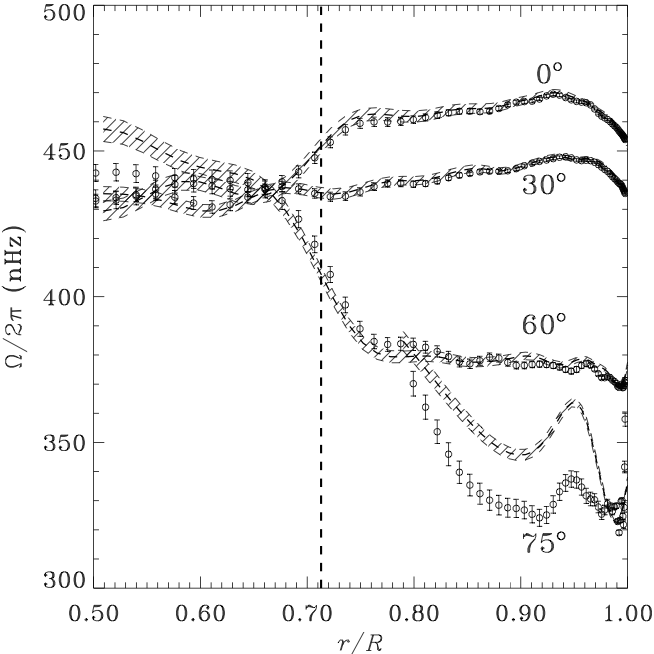
\includegraphics[keepaspectratio,width=0.8\textwidth]{invertedrotation}
\caption{Inversione della velocit\'a di rotazione a diverse latitudini. La linea verticale tratteggiata indica la base della zona convettiva. Da \cite{chr02helioseismology}.}
\end{figure}

Considero la correzione al primo ordine in $\Omega$. Il campo di velocit\'a rotazionale in coordinate sferiche \'e 
\begin{align}
&\vec{v_0}=(0,0,r\Omega\sin{\theta})=\vecp{\Omega}{r}\\
&\vec{\Omega(r,\theta)}=(\Omega(r,\theta)\cos{\theta},-\Omega(r,\theta)\sin{\theta},0)
\end{align}

In assenza di moti macroscopici il termine d'inerzia \'e $\rho_0\TDy{t}{\vec{v}}=\rho_0\PtwoDy{t}{\vec{\xi}}$, mentre in caso di rotazione si ha
\begin{equation}
\rho_0(\PDof{t}+\scap{v_0}{\nabla})^2\vec{\xi}
\end{equation}

Considero il termine dovuto alla rotazione come una piccola correzione alle frequenze dei modi
\begin{align}
&\omega_{(l,m)}+\Delta\omega_{(l,m)}&\intertext{quindi l'equazione del moto al primo ordine nella perturbazione, con $\alpha=(l,m)$, \'e}\nonumber\\
&\rho_0(\omega_{\alpha}^2+2\omega_{\alpha}\Delta\omega_{\alpha})\vec{\xi}=\nabla P_1-\frac{\rho_1}{\rho_0}\nabla P_0+\rho_0\nabla\Phi_1+2i\omega_{\alpha}\rho_0(\scap{v_0}{\nabla})\vec{\xi}\\
&\intertext{da cui si deduce}\nonumber\\
&\Delta\omega_{\alpha}=\frac{i\int\rho_0\xi_{\alpha}^*(\scap{v_0}{\nabla})\xi_{\alpha}}{\int\rho_0\xi_{\alpha}^*\xi_{\alpha}}=\frac{-m\int\rho_0\Omega\xi_{\alpha}^*\xi_{\alpha}\,dV+i\int\rho_0\xi_{\alpha}^*(\vecp{\Omega}{\xi_{\alpha}})\,dV}{\int\rho_0\xi_{\alpha}^*\xi_{\alpha}}
\end{align}

Il problema di trovare $\Omega(r,\theta)$ dalla differenza $\Delta\omega_{\alpha}$ \'e lineare in $\Omega$ quindi $\Delta\omega_{\alpha}\propto\Omega$. Per determinare quindi la rotazione dobbiamo conoscere l'autovalore $\xi_{\alpha}$ dello stato imperturbato.

%Per rotazione puramente radiale $\Omega(r)$ la relazione tra lo splitting delle frequenze e la rotazione \'e
%\begin{equation}
%\Delta\omega_{\alpha}=-m\frac{\int_0^{\rsun{}}\rho_0\Omega\{|\xi_r-\xi_h|^2+[l(l+1)-2]|\xi_h|^2\}r^2\,dr}{\int_0^{\rsun{}}\rho_0\{|\xi_r|^2+l(l+1)|\xi_h|^2\}r^2\,dr}=\int_0^{\rsun{}}K_{\alpha}(r)\Omega(r)\,dr
%\end{equation}
%Any given $\Delta\omega_{\alpha}$ samples angular velocity in the depth range corresponding to $\xi_{\alpha}$.

La velocit\'a angolare contribuisce a $\Delta\omega_{\alpha}$ negli strati in cui $\xi_{\alpha}$ \'e apprezzabile. Nel caso di rotazione dipendente solo da r si ha che $\Delta\omega_{\alpha}$ \'e lineare in m: ho $2l+1$ frequenze equispaziate.



%%% SOS
%\part{INVERSIONE SOS}
%\section{Osservabili stellari/demo beamer}

\begin{frame}<1>[label=noinside]{Modello stellare}{Come indagare la fisica interna a una stella?}

\onslide<1->\begin{block}{Osservabili stellari:}
$L$, $M$, $R$, $T_e$, $(\frac{Z}{X})_{ph}$, $g_{ph}$.
\end{block}

\onslide<1->\begin{block}{Informazioni sulla struttura interna?} Condizione di equilibrio idrostatico
\end{block}

%Teorema Vogt-Russel: $X_i(r)$, $M$ \pause equilibrio (idrostatico/termico) determinano struttura stellare .
%\pause

\onslide<1->\begin{block}{Modello stellare: diagramma di \hr{}.}
\end{block}

\onslide<2->\begin{block}{Descrizione fisica interno stellare: parametri aggiuntivi}
Convezione, diffusione e sedimentazione elementi pesanti, equazione di stato, opacit\'a
\end{block}

\onslide<2->\begin{block}{Astrosismologia}
Restringo spazio parametri sistemi stellari lontani
\end{block}

\end{frame}

{ % all template changes are local to this group.
    \setbeamertemplate{navigation symbols}{}
    \begin{frame}[plain]{Diagramma di \hr{}}
        \begin{tikzpicture}[remember picture,overlay]
            \node[at=(current page.center)] {
                %\includegraphics[width=\paperwidth]{yourimage}
            };
        \end{tikzpicture}
     \end{frame}
}
\againframe<2>{noinside}

\section{Inversione della legge di Duvall}

\section{Inversione non asintotica}

\section{Vincoli al modello solare dalle osservazioni sismologiche}


\end{document}